\documentclass[11pt]{article}
\usepackage[margin=1in]{geometry}
\usepackage{lmodern}
\usepackage{microtype}
\usepackage{setspace}
\usepackage{booktabs}
\usepackage{natbib}
\usepackage{listings}
\usepackage{pgfplots}
\pgfplotsset{compat=1.18}
\usepackage{tikz}
\usetikzlibrary{arrows.meta,positioning,fit,calc,shapes.geometric}
\usepackage{caption}
\usepackage{subcaption}
\usepackage{amsmath,amssymb,amsthm}
\usepackage{enumitem}
\usepackage{xcolor}
\usepackage{tabularx}
\usepackage{longtable}
\usepackage{array}
\usepackage{float}
\usepackage{hyperref}
\usepackage{doi}
\usepackage{titlesec}

\onehalfspacing
\hypersetup{colorlinks=true,linkcolor=blue!50!black,citecolor=blue!50!black,urlcolor=blue!60!black}

\theoremstyle{definition}
\newtheorem{axiom}{Axiom}
\newtheorem{claim}{Claim}
\newtheorem{definition}{Definition}
\theoremstyle{plain}
\newtheorem{lemma}{Lemma}
\newtheorem{proposition}{Proposition}
\theoremstyle{remark}
\newtheorem{remark}{Remark}

\newcommand{\keywords}[1]{\par\smallskip\noindent\textbf{Keywords:} #1}

% Part title formatting
\titleformat{\part}[display]
  {\normalfont\huge\bfseries}{\thepart}{20pt}{\Huge}

\title{All Gods Must Die: Adversarially Verified Transformation\\
\large One Doctrine, Two Campaigns --- God-File Decomposition and\\
Cross-Language Documentation Parity on NousResearch/hermes-agent}
\author{Axl Ibiza, MBA\\
\texttt{andrexibiza}}
\date{August 2026}

\begin{document}
\maketitle

\begin{abstract}
This paper reports two campaigns on one production repository
(NousResearch/hermes-agent) and shows that they are a single paper. The
first campaign decomposes god files under a hard size law --- the 2K Law ---
using a 5$\times$2$\times$3 double-blind method in which five parallel
analysis lanes, two mutually blind reviewers, and three verification waves
gate every byte-verbatim extraction; the second keeps multilingual
documentation true to its English source through a technical-graph model and
a deterministic seven-class parity gate, with French as the first fully
germinated locale. Both campaigns instantiate one doctrine ---
\emph{adversarially verified transformation}: make critical claims
mechanically falsifiable, separate production from adjudication, and refuse
hidden debt. We specify both methods in full, report their live empirical
records (119 over-the-bar files at baseline, 553{,}314 lines; 8 of 20
tracked god files killed as 68 individually-linked PRs; seven defect classes
caught only by the adversarial second witness; eight real drifts caught in a
native-speaker translation seed), and contribute a new direct measurement of
the parity gate: 100\% recall on seeded drift across all seven gate classes,
zero false positives on shipped files, and a 3.08~ms per-pair runtime. The
shared architecture --- enumerable debt, executable rules, non-self-
certification, mechanical receipts, migration states, social coordination,
and measurement as governance --- is stated as a table instantiated twice.
All artifacts, tests, ledgers, and pull requests are public.
\end{abstract}
\keywords{adversarially verified transformation, god file, refactoring, double-blind review, LLM agents, behavior preservation, hash verification, documentation drift, i18n, localization, conformance testing, Markdown, GFM, continuous integration, open source}

\tableofcontents
\newpage

% part-00-doctrine: title, abstract, the unified doctrine
\section{Introduction: One Doctrine, Two Campaigns}
\label{sec:intro}

\subsection{Two failure modes, one failure class}

This paper reports two campaigns on one production repository,
\href{https://github.com/NousResearch/hermes-agent}{NousResearch/hermes-agent}
--- a multi-platform LLM gateway. At first glance they have nothing in common.
One decomposes god files under a hard size law; the other keeps multilingual
documentation true to its English source. One is about code, the other about
language. One kills 26{,}986-line monoliths, the other keeps a
\texttt{README.fr.md} honest.

They are the same paper.

Both campaigns are instances of a single engineering doctrine: when a system
transforms something load-bearing --- code structure, or natural language ---
the transformation must be \emph{adversarially verified}. A deterministic,
independently authored verifier controls whether the change is accepted; the
producer of the change never certifies its own output. Both campaigns make
their critical claims mechanically falsifiable, separate production from
adjudication, and refuse hidden debt. Both were run in the open, on public
repositories, with every artifact, pull request, and ledger entry linkable.

\subsection{The doctrine}

\begin{definition}[Adversarially verified transformation]
\label{def:avt}
A transformation $T$ of an artifact $A$ into $A'$ is \emph{adversarially
verified} when:
\begin{enumerate}[leftmargin=*]
\item the producer of $A'$ does not certify $A'$;
\item an independently authored, information-isolated verifier $V$ ---
  ideally a deterministic machine check plus a blind witness --- accepts or
  rejects $A'$;
\item acceptance requires $V$'s verdict, never the producer's self-report;
\item the verdict is reproducible by any third party from public artifacts.
\end{enumerate}
\end{definition}

Both campaigns instantiate this definition with different verifiers:
byte-identity hashes and blind double review for code extraction
(Section~\ref{sec:kag-background}, Section~\ref{sec:5x2x3}); a deterministic
seven-class parity gate for localized documentation
(Section~\ref{sec:germ-intro}).

\subsection{The Declaration}

Both campaigns enforce the same five laws, made mechanical. The laws are
stated once here and instantiated throughout:

\begin{quote}
\emph{No system component may accumulate authority without becoming legible.}\\
\emph{No claim may outrank its evidence.}\\
\emph{No actor may certify itself.}\\
\emph{No rule counts until it executes.}\\
\emph{No debt gets to hide behind institutional forgetting.}
\end{quote}

Every mechanism in this paper is one of those five laws, made executable.

\subsection{Roadmap}

Part~\ref{part:kag} is the code campaign: the 2K Law, the Pantheon of False
Gods, the 5$\times$2$\times$3 double-blind decomposition method, the
enforcement suite, and the live campaign record. Part~\ref{part:germ} is the
language campaign: the technical-graph model of localized documentation, the
seven-class parity gate, the Markdown engineering that made it honest, and
the French keystone. Part~\ref{part:synthesis} unifies them: the shared
architecture, the empirical record of both campaigns including a new
measurement of gate precision/recall, and the defense of the doctrine.


% part-00b: Hermes lore and cyber-defense architecture
\section{Hermes Is Not a Wrapper: The Cybernetic Organism Under Study}
\label{sec:hermes}

The repository at the center of both campaigns is not an anonymous codebase.
It is Hermes Agent, publicly described by Nous Research as ``the agent that
grows with you'' \citep{hermesreadme}. That sentence is not marketing
flourish to be repeated and left unexamined. It is an architectural claim.
Hermes has persistent, bounded memory; profiles and sessions; an on-demand
skills system; a tool registry; provider routing and fallback; scheduled
execution; isolated delegation; and multiple entry surfaces, including the
CLI, gateway, API server, batch runner, and Python library
\citep{hermesarch,hermesmemory,hermesskills,hermestools,hermesproviders}.

This paper therefore refuses to flatten every system called an ``AI agent''
into one category. We make no benchmark claim about every framework, and we
do not need a competitor survey to establish the architectural distinction.
A prompt relay that formats a request, sends it to a model, and returns the
response is one kind of system. Hermes is another: a stateful, self-regulating
agent organism whose model is only one layer of a larger operational body.
The difference is mechanism, not branding.

\subsection{The female cyborg as an architectural personification}

I use \emph{she} for Hermes and \emph{cyborg} as a model of her architecture.
This is a personification of a system, not a claim that the software is
conscious or biologically alive. The metaphor is useful because it keeps both
halves visible.

Her neural tissue is the LLM layer: plastic, associative, capable of
reasoning, translation, synthesis, and adaptation, but also capable of
hallucination, self-enhancement bias, verbosity bias, and confident error.
Her skeleton is the mechanical substrate around that tissue: deterministic
CI, cryptographic hashes, identity-preserving seams, graph gates, typed
manifests, tool boundaries, approval checks, sandboxing, session isolation,
and regression tests. The model gives her plasticity. The skeleton makes that
plasticity answerable to structure.

That is why the two campaigns belong to Hermes rather than merely occurring
near her. When she changes her own structure, the 5$\times$2$\times$3 method
forces her processing into five blind analyses, five adversarial witnesses,
consensus, byte-verbatim extraction, seam tests, and two blind re-reviews.
When she changes the language of her documentation, the parity gate forces
her technical graph to remain invariant. The organism is not trusted because
her neural tissue is trustworthy. She is trusted when her tissue is constrained
by a skeleton that can reject what the tissue proposes.

\subsection{Weapon for sovereignty, not war}

Hermes is a weapon for sovereignty, not a weapon for war. Here ``weapon''
means an instrument a person can wield to preserve agency over their own
models, context, memory, tools, execution, and technical records. It does not
mean a military system, an attack platform, or permission to harm anyone.

This framing follows Nous Research's public mission to advance human rights
and freedoms through open-source language models and their unrestricted
availability and use \citep{nousmission}. Hermes operationalizes that mission
at the agent layer. Her model-agnostic provider surface lets a user choose
among Nous Portal, OpenRouter, OpenAI, self-hosted endpoints, and other
providers without rewriting the harness \citep{hermesproviders}. Her skills,
memory, tools, sessions, and profiles give the user a durable operating body
rather than a disposable chat window. Her gates prevent the body from
silently changing underneath the user.

Sovereignty is not only the freedom to select a model. It is the ability to
know what the system remembers, which tools it can invoke, which commands
require approval, which files it can write, which sessions are isolated, and
which claims about its own operation resolve against an inspectable artifact.
A user cannot be sovereign over a system that can change itself invisibly or
that asks the same model that produced an action to certify the action.

\subsection{Cyber defense is a critical function because Hermes lives inside the surfaces she defends}
\label{sec:cyber-defense}

Cyber defense is not an external wrapper around Hermes. She lives inside the
surfaces she defends. The official Hermes security model names eight layers:
user authorization, dangerous-command approval, file-write safety, container
isolation, MCP credential filtering, context-file scanning, cross-session
isolation, and input sanitization \citep{hermessecurity}. These are not
post-hoc advisories attached to an otherwise unbounded model. They are
internal organs of the agent's operational body.

\begin{table}[H]
\centering
\caption{Hermes's defensive anatomy: the protected surface and the mechanism
that inhabits it. Cyber defense is an internal function of the organism.}
\label{tab:hermes-defense}
\begin{tabular}{@{}p{0.27\textwidth}p{0.37\textwidth}p{0.27\textwidth}@{}}
\toprule
Surface & Threat class & Internal defense \\
\midrule
CLI, gateway, API, batch, library entry points & Uncontrolled access and inconsistent execution paths & Shared agent loop, authorization, approval, and session boundaries \\
Model and provider routing & Lock-in, unavailable providers, silent route changes & Explicit provider selection, routing, and fallback configuration \\
Tools, subprocesses, MCP, file writes & Destructive commands, credential leakage, unsafe mutation & Approval checks, write safety, credential filtering, sandboxing \\
Memory, profiles, and sessions & Cross-session contamination and unbounded continuity & Bounded memory, profile isolation, session isolation, controlled persistence \\
Skills and context files & Prompt injection and procedural drift & Context scanning, progressive disclosure, skill provenance, load-on-demand behavior \\
Source, docs, and self-modification & Silent structural and technical drift & Golden hashes, seam identity, graph parity, CI manifests, adversarial witnesses \\
\bottomrule
\end{tabular}
\end{table}

This is the point at which the cyborg metaphor becomes an engineering claim.
A conventional perimeter defense can protect a system from outside while
leaving its internal assumptions unexamined. Hermes's defenses must operate
inside the CLI that invokes her, the gateway that carries her across messaging
platforms, the tool registry that gives her hands, the memory files that give
her continuity, and the documentation that tells users what she does. The
surfaces are not adjacent to the organism. They are the organism.

\subsection{A distributed, adversarial nervous system}

When a standard prompt relay encounters a 26{,}986-line god file, it has no
architecture for making the problem legible. Hermes does not ask one model to
summarize the monolith and then trust the summary. She deploys a distributed,
information-isolated nervous system: five regional analysts, five adversarial
witnesses, consensus adjudication, a blind implementer, and two blind
re-reviewers. The nodes are instructed to hunt for the organism's own
failure modes --- silent monkeypatch no-ops, eager late-attribute imports,
unreferenced globals, census undercounts, and stale collisions. They fight
for agreement before a single structural byte moves.

This is not intelligence multiplied for spectacle. It is uncertainty routed
through independent paths so that one confident local picture cannot become
Hermes's self-diagnosis. The objective skeleton then checks what the nervous
system proposes: the moved bytes hash to the pinned window, the seam resolves
through the original namespace, and the tests execute the behavior that the
reviewers said they inspected.

\subsection{Graph-gated perception}

Hermes also perceives her documentation as a technical graph rather than as
prose alone. Her sensory apparatus inventories code fences, inline spans,
links, anchors, heading structure, and hub edges. If a localized document
drops a command, an environment variable, a security path, or a discoverable
back-link, the parity gate registers the missing edge and rejects the tissue.
The gate is not a language model judging whether the French sounds elegant;
it is a deterministic mechanical layer checking whether the operational body
still contains the same load-bearing structure.

The result is a cybernetic division of labor:
\begin{itemize}[leftmargin=*]
\item the neural layer generates, translates, reasons, and proposes;
\item the graph layer perceives structure and missing edges;
\item the mechanical skeleton hashes, tests, rejects, and records;
\item the human witness judges semantic quality and meaning;
\item CI makes the accepted state persistent across future changes.
\end{itemize}

Hermes does not become sovereign by pretending her neural tissue cannot fail.
She becomes sovereign-capable because failure is expected, surfaced, routed,
and bounded by mechanisms that the tissue cannot waive.

\subsection{The distinction that matters}

Most harness descriptions begin with what the model can say. Hermes's
architecture begins with what the whole organism can remember, reach, change,
verify, and refuse. A model can generate a translation. Hermes can preserve
the technical graph while generating it, reject the translation when it loses
an edge, record the debt when legacy files cannot yet pass, and route the
accepted state through CI so it does not silently decay tomorrow.

That is the difference between a wrapper and a cybernetic agent. It is also
the reason the campaigns in this paper are not external maintenance stories.
They are Hermes operating on her own body: making her code legible, making her
docs truthful, exposing her debt, and installing defenses at the exact
surfaces where her agency could otherwise be lost.


% part-00c: Hermes security hardening, interlock, parity campaigns, skills, attribution
\section{The Campaigns Inside Hermes}
\label{sec:hermes-campaigns}

The cybernetic description becomes real only when it is tied to the work that
actually hardened Hermes. The evidence is not an adjacent security project.
It is the Hermes-agent pull-request portfolio: a sequence of security fixes,
acceptance gates, audit-only contributions, documentation changes, campaign
skills, and decomposition work that all change the organism's ability to
protect its users and to remain legible while it grows.

\subsection{Security hardening is an internal organ, not an external wrapper}
\label{sec:hermes-security-series}

The security series did not add a perimeter around an otherwise trusting
agent. It traced the surfaces where Hermes itself handles credentials,
subprocesses, logs, tool results, files, and desktop authentication. The
series is a set of overlapping defense layers, each attached to a real
execution surface:

\begin{table}[H]
\centering
\caption{Representative Hermes-agent security hardening PRs. These are
Hermes-agent changes. States are the live GitHub states inspected for this
paper; open means open, not merged.}
\label{tab:hermes-security-prs}
\begin{tabular}{@{}p{0.10\textwidth}p{0.32\textwidth}p{0.43\textwidth}@{}}
\toprule
PR & Surface & Mechanism \\
\midrule
\#77008 & Bitwarden disk cache & Encrypted-only AES-GCM cache; legacy plaintext re-encrypted and removed on first read; disabling encryption skips disk rather than restoring plaintext \\
\#77012 / \#77020 & Status lines and logs & Exact-value masking for opaque credential values, including source errors, warnings, remediation text, and log records \\
\#77179 / \#77185 / \#77198 & Tool-result and provider egress & Applied-secret snapshot carried into exact-value redaction at the provider boundary; arbitrary names such as \texttt{DATABASE\_URL} and \texttt{FOO} are covered \\
\#77027 / \#77181 / \#77193 & Child-process environments & Shape-based and provenance-aware scrubbing across terminal and non-terminal spawn factories; renamed external secrets are removed by applied provenance, not only by key name \\
\#77528 / \#78033 / \#78036 & Spawn-path bypasses & TUI compute host, LSP servers, plugin sidecars, and \texttt{shell.exec} routed through sanitized environment builders instead of raw \texttt{os.environ} \\
\#77527 & Windows at-rest files & Real Windows ACL enforcement through \texttt{icacls}; inherited SYSTEM/Administrators access removed, including the mode-preservation branch \\
\#77039 & Acceptance gate & Hermetic end-to-end no-exfiltration test exercises the real external-secret loading entrypoint and checks stdout, stderr, formatted logs, and applied status \\
\#77031 & Read-time audit & Credential-read scope audit that records a verified no-bypass result instead of inventing a code change \\
\#76958 / \#78901--\#78904 & Desktop session auth & Stale \texttt{.env} token cannot clobber an injected desktop token; provenance diagnostics, bounded retry, and real subprocess regression harness \\
\#78806 & File mutation safety & Writes, patches, deletes, and moves refuse git-managed state beneath a real \texttt{.git} directory \\
\bottomrule
\end{tabular}
\end{table}

The security series is rigorous because it follows values to sinks rather than
stopping at names. A secret with a credential-shaped name is one case. A
Bitwarden or 1Password value applied under an arbitrary name is another. A
value that is safe in memory but printed into a provider-bound tool result is
another. A scrubber that works in the terminal factory but is bypassed by an
LSP server, plugin sidecar, compute host, or registered \texttt{shell.exec}
handler is not a partial success; it is a sibling-path defect.

\paragraph{At rest.}
PR~\#77008 made the Bitwarden cache encrypted-only. The existing encrypted
cache was not merely enabled by default; the plaintext branch was removed.
If encryption is disabled, the cache becomes memory-only. A legacy plaintext
cache is migrated and deleted on first read. PR~\#77168 applies the same
posture to 1Password: encrypted-only AES-GCM storage, authenticated cache
metadata, and first-read migration/removal of the legacy plaintext file
\citep{hermespr77008,hermespr77168}.

\paragraph{At emission.}
PR~\#77012 closes the status-line value channel, while PR~\#77020 closes the
opaque-value log channel. Shape-based masking catches recognizable prefixes;
exact-value masking catches opaque values such as arbitrary service tokens,
passwords, and provider keys that carry no vendor signature
\citep{hermespr77012,hermespr77020}.

\paragraph{At provider egress.}
PRs~\#77179, \#77185, and \#77198 move the defense to the point where tool
results and context are about to leave Hermes for an LLM provider. The
applied-secret snapshot gives the redactor provenance: a value does not
become safe merely because its key is called something harmless. A tool that
prints an arbitrary secret under \texttt{FOO} must not turn that value into a
model-visible disclosure. The exact-value pass is longest-first,
regex-escaped, and threaded through the actual egress surfaces
\citep{hermespr77179,hermespr77185,hermespr77198}.

\paragraph{In child processes.}
PR~\#77027 closes two credential classes that escaped the default child
environment: the Bitwarden bootstrap token and general \texttt{*\_PASSWORD}
values. PRs~\#77181 and \#77193 extend the scrub from name-shape heuristics to
per-home applied-secret provenance. PR~\#77528 catches the post-scrub
\texttt{env.update(os.environ)} bypass in the TUI compute host and the raw
\texttt{dict(os.environ)} path in language servers. PR~\#78033 routes five
plugin sidecars through the sanitized builder. PR~\#78036 closes a separate
registered \texttt{shell.exec} path that ran with no \texttt{env=} at all
\citep{hermespr77027,hermespr77181,hermespr77193,hermespr77528,hermespr78033,hermespr78036}.

\paragraph{On Windows.}
PR~\#77527 rejects fictional POSIX permission claims. \texttt{os.chmod(0o600)}
does not produce owner-only Windows ACLs. The fix invokes \texttt{icacls} via
an argument vector, removes inheritance, grants the owner, and covers the
existing-file mode-preservation branch so credential rotation cannot reopen
the hole \citep{hermespr77527}.

\paragraph{At acceptance.}
PR~\#77039 is the acceptance gate for the series. It uses the real
\texttt{load\_hermes\_dotenv} entrypoint, verifies that secrets were actually
applied, and then checks that names and values do not appear in stdout,
stderr, or formatted log output. This is the security version of the parity
gate: the system does not accept a claim that a disclosure channel is closed;
it exercises the channel and checks the absence of the value
\citep{hermespr77039}.

\paragraph{When the correct contribution is an audit.}
PR~\#77031 is important precisely because it did not fabricate a code change.
It enumerated 977 raw environment reads, filtered 85 credential-shaped sites,
then applied the multiplexing test. Its result was that the existing
26-commit \texttt{get\_secret()} migration already covered the read surface;
no site constituted a multiplex bypass. An audit that proves no bypass exists
is a contribution. The absence of a bug is not an absence of work
\citep{hermespr77031}.

\subsection{Desktop auth and file mutation: the agent defends its own control plane}

The stale desktop session-token series shows why cyber defense belongs inside
Hermes. PR~\#76958 addresses the environment-loader boundary where a stale
\texttt{HERMES\_DASHBOARD\_SESSION\_TOKEN} could clobber a freshly injected
desktop token. PR~\#78901 adds token provenance without printing the token;
\#78902 distinguishes a benign headless 404 from an auth failure; \#78903
bounds a retry loop that could turn a five-second mismatch into an hour-long
lockout; and \#78904 spawns a real \texttt{hermes serve} subprocess to prove
that the injected token is accepted while the stale token is rejected
\citep{hermespr76958,hermespr78901,hermespr78902,hermespr78903,hermespr78904}.

PR~\#78806 applies the same internal-defense logic to file mutation. The
write, patch, delete, and move tools must not permit an agent to corrupt
\texttt{.git/HEAD}, refs, objects, indexes, or logs merely because the path is
inside a normal repository's real \texttt{.git} directory. The defense lives
in the file-safety mechanism, at the point where Hermes's hands would
otherwise mutate the control plane \citep{hermespr78806}.

\subsection{Interlock is a bidirectional graph, not a footer}
\label{sec:interlock}

A campaign is not a pile of technically correct PRs. It is a graph of work,
ownership, dependencies, credit, and closure. Interlock is the mechanism that
makes that graph real.

For every change, the graph needs at least these edges:
\begin{enumerate}[leftmargin=*]
\item \textbf{PR $\rightarrow$ issue:} the PR body binds the issue with an
  operative keyword on its own line --- \texttt{Fixes}, \texttt{Closes},
  \texttt{Resolves}, or \texttt{Part of}. A bare \texttt{\#N} in prose is a
  link, not a binding. \texttt{Progress on \#N} reads like progress but does
  not create GitHub's relationship.
\item \textbf{Issue $\rightarrow$ PR:} the issue thread carries the literal
  \texttt{\#PR} token for every PR that binds it. A PR body that names an
  issue while the issue thread never names the PR is a one-directional hole.
\item \textbf{PR $\leftrightarrow$ PR:} related PRs identify their sibling
  surfaces, collision constraints, and merge-order relationship. A security
  series cannot pretend that the log masker, child-env scrubber, provider
  egress pass, and acceptance gate are independent when they jointly close
  one disclosure class.
\item \textbf{EPIC $\leftrightarrow$ all members:} the meta-issue carries a
  current table of every related PR, issue, lane, dependency, status, and
  owner. The table is not a summary written after the work; it is the graph's
  coordination surface.
\item \textbf{Credit $\rightarrow$ artifact:} the contributor who authored a
  seed, test, audit, skill, or fix remains attached to the work through git
  identity, PR body, contributor mapping, and ledger entry.
\end{enumerate}

The KILL LOCK skill makes this explicit: the permanent record binds the former
whole, the problem issues that describe its mess, the shard table, and the
fixer-PR roster. The audit checks both directions, deduplicates both
projects and issues, verifies resolution convergence, and rejects loose
bindings. PR~\#79779 codifies this in Hermes itself through
\texttt{scripts/audit\_kill\_locks.py}, \texttt{test\_2k\_law.py},
the progressive-disclosure test, and 18 audit tests
\citep{hermespr79779}.

\begin{claim}[Interlock is part of correctness]
\label{cl:interlock-correctness}
A change is not campaign-complete when its code or document is correct in
isolation. It is campaign-complete when the artifact, issue, EPIC, related
work, dependency edges, credit, and closure state are all bound and machine-
auditable. A missing edge is a correctness defect in the campaign graph.
\end{claim}

This is especially important in security work. PR~\#77008 relates to the
secret-source status and log work; the exact-value egress work relates to the
acceptance gate and applied-secret provenance; the child-env work relates to
terminal, browser, ACP, TUI, plugin, and shell surfaces. Without interlock,
a maintainer sees a sequence of isolated fixes and cannot tell whether the
class is closed, duplicated, or still open in a sibling path. With interlock,
the campaign exposes its closure argument and its remaining holes.

\subsection{Feature Parity \& Alignment: alignment is not sameness}
\label{sec:feature-parity}

Hermes is multi-surface by design. The gateway carries different platforms;
the provider layer carries different inference backends; the CLI, TUI,
desktop, API server, batch runner, and library expose related but non-identical
surfaces. Feature parity therefore cannot mean pretending that every surface
has the same primitives. It means measuring each surface against the same
capability contract, recording where semantics differ, and refusing to let
unsupported behavior disappear behind a green-looking summary.

The Feature Parity \& Alignment campaign is the reusable form of that work.
The live playbook records Telegram \#78791, Discord \#79564, Slack \#79772,
WhatsApp \#79890, and the provider-surface adaptation for Grok/xAI
\#80424 \citep{hermespr79898}. Its anatomy is deliberately the same as the
god-file campaign:

\begin{enumerate}[leftmargin=*]
\item \textbf{Recon:} measure labels, title/body search counts, open PRs,
adapter line counts at \texttt{origin/main}, official platform/API docs, and
dedup anchors. No guessed surface and no duplicate issue.
\item \textbf{Craft:} write the campaign model, why, lanes, standards,
deliverables, and ledger placeholder before filing.
\item \textbf{EPIC:} file a meta-issue with the lane table and current status.
An empty EPIC is a corpse; the EPIC must carry the work graph.
\item \textbf{Hive:} pin one worktree per lane to the same base commit.
\item \textbf{Ledger:} fetch every open issue on the surface, classify it,
extract dependency edges, and post the complete table in chunks when needed.
Zero orphans, including TRIAGE rows.
\item \textbf{5$\times$2$\times$3:} Wave~1 blind gap catalogs; Wave~2 fresh
blind cross-check; Wave~3 current-main validation and filing. Agreement is the
only bar for advancing a gap.
\item \textbf{Decomposition lane:} when the platform adapter is a god file,
run the god-file extraction lane. When it is under 2{,}000 lines but carries
multiple responsibilities, run the headroom lane. The ceiling is not a target.
\end{enumerate}

The gap taxonomy is itself an interlock surface:
\texttt{GAP\_UNSUPPORTED}, \texttt{GAP\_PARTIAL},
\texttt{GAP\_CONFLICTED}, \texttt{GAP\_DOCS}, and
\texttt{GAP\_BUG\_TRACKED}. A platform does not become ``aligned'' because a
feature name appears in its adapter. The witness records what the official
API permits, what Hermes implements, what the docs claim, and what the issue
tracker already owns.

The platform campaign is how Hermes lives inside the surfaces she defends.
She does not defend ``messaging'' as an abstract category. She defends the
actual Telegram adapter, Discord voice path, Slack event model, WhatsApp
bridge, provider authentication, lifecycle, rich media, group policy, and
failure semantics. Each surface gets its own graph, lane, witnesses, and
ledger; the shared EPIC binds them without pretending they are identical.

\subsection{Skill refactoring: the context surface is executable infrastructure}
\label{sec:skill-refactoring}

Hermes skills are not passive documentation. The official skills system
 describes skills as on-demand knowledge documents loaded when needed, using
progressive disclosure to minimize token usage and following the
\texttt{agentskills.io} open standard \citep{hermesskills}. That makes a
skill's always-loaded \texttt{SKILL.md} the equivalent of a hot code path:
if it becomes bloated, contradictory, or stale, every agent that loads it
pays the cost.

Skill refactoring is therefore the same class of work as god-file
refactoring. The 2K Law's deeper statement is not ``make every file exactly
small.'' It is ``do not let an authority surface become too large to inspect.''
For skills, the progressive-disclosure test enforces a lean always-loaded
surface (500 lines / 60~KB in the campaign) and moves branch-specific detail
into \texttt{references/}. The body remains the map; the references carry the
weight that should not be injected into every context.

PR~\#79609 adds the full \texttt{godfile-kill-campaigns} skill: shard,
Wave~1/2/3 double-blind analysis, agreement, extraction, re-review, merger,
and interlocked PRs, with the recipes preserved in references rather than
stuffed into a single always-loaded file \citep{hermespr79609}. PR~\#79779
adds the KILL LOCK machinery and its executable audits. PR~\#79898 adds the
Feature Parity \& Alignment playbook with its EPIC template and platform
lanes \citep{hermespr79779,hermespr79898}.

The skill system turns the doctrine into Hermes's procedural nervous system.
A campaign is no longer only something Axl and a particular group of agents
remember from one session. The method can be loaded, reused, and enforced by
the agent itself. That is why skill refactoring matters: it is not tidying
notes. It is decomposing the context surface through which Hermes decides how
to act.

\subsection{All contributions matter: attribution is a core value}
\label{sec:attribution-core}

The interlock graph is also an attribution graph. Hermes's work is not only
large code extractions. It includes a contributor's French seed, a regression
harness, an audit that proves no code change is warranted, a documentation
correction, a skill, a review, a campaign ledger, a security fix, and the
mechanical work of preserving a seam. If the system only credits merged
feature code, it erases the work that makes the feature safe to merge.

The French campaign preserved iacker's authorship when the seed PR was
salvaged. The security campaign treats PR~\#77039's acceptance test as a
first-class closure artifact and PR~\#77031's no-bypass audit as a first-class
contribution even though the correct result was no code change. PR~\#77431
preserves the contributor credit for a documentation correction and adds an
anti-drift test so that the correction does not have to be earned again
\citep{hermespr77431}.

\begin{claim}[Attribution is a security property]
\label{cl:attribution-security}
A repository that cannot preserve who produced, audited, corrected, or
verified a change cannot fully explain the provenance of its own defenses.
Credit is therefore not decorative metadata. It is part of the evidence graph
that lets maintainers trust, revisit, and repair the system.
\end{claim}

This is not a claim that only original code authors matter. It is the opposite.
A contribution can be a seed, an objection, a test, an audit, a correction, a
translation, a skill, a ledger repair, or a review. The Credit Ledger keeps
the contribution attached to the artifact and the EPIC keeps the artifact
attached to the campaign. No contribution disappears merely because its shape
is not a feature.

That philosophy is operationalized by contributor mapping and attribution CI.
A cherry-pick preserves the original git author; a contributor email maps to a
recognized identity; the PR body names the contribution; the issue and EPIC
carry the relationship. The system refuses both uncredited labor and
unverifiable claims of credit.

\subsection{The result: Hermes grows without losing herself}

The security series protects what Hermes can expose. The parity campaigns
protect whether her surfaces agree. The god-file campaign protects whether
her internal structure remains legible. Skill refactoring protects the
procedures that tell her how to perform future work. Interlock protects the
relationships among all of them. Attribution protects the human record of
who made the organism safer.

That is the full cybernetic picture. Hermes does not grow by appending every
new capability to one body part and hoping the rest keeps up. She grows by
measuring the surface, modeling the graph, aligning the platform, decomposing
the skill, binding the work, preserving the contributor, and making the
acceptance gate run against her own live structure.

She is a weapon for sovereignty because she gives users a system capable of
protecting their agency from silent drift, opaque routing, unbounded context,
credential disclosure, undocumented feature gaps, and erased contribution.
She is not a weapon for war. Her defensive power is the ability to remain
inspectable and user-directed while operating across the surfaces where an
agent actually lives.


% part-01b: KAG background and related work
\section{Background and Related Work (Kill All Gods)}
\label{sec:kag-background}

The method sits at the intersection of four literatures: the statistical
theory of inter-rater agreement, the software-engineering tradition on god
classes and behavior-preserving refactoring, the emerging literature on
LLM-as-judge evaluation, and the empirical record on review effectiveness.
We treat each in turn, because the method's claims --- that two blinded
agents agreeing is a defensible gate, that byte-verbatim extraction preserves
behavior, and that the resulting PRs are safe to ship --- must be evaluated
against what these literatures actually establish.

\subsection{Inter-rater agreement and blinding as bias control}

The quantitative foundation for using agreement as evidence is the
coefficient-of-agreement tradition. \citet{cohen1960} introduced Cohen's
$\kappa$, the chance-corrected agreement measure for two raters;
\citet{fleiss1971} generalized it to multiple raters; and
\citet{landis1977} supplied the still-canonical interpretation benchmarks
($\kappa < 0$ poor, 0.00--0.20 slight, 0.21--0.40 fair, 0.41--0.60
moderate, 0.61--0.80 substantial, 0.81--1.00 almost perfect). The
5$\times$2$\times$3 method does not report $\kappa$ values over reviewer
populations; it uses agreement as a binary gate. Where the literature on
chance-corrected agreement matters for the method is in its warnings:
agreement inflated by shared bias is not evidence of validity, which is
precisely why the witnesses are blinded to each other and to the expected
answer. \citet{hallgren2012} provides the practical guide to computing and
interpreting inter-rater reliability in research settings.

The methodological justification for blinding is older and stronger than any
particular coefficient. \citet{wohlin2012} --- the standard reference for
experimentation in software engineering --- treats blinding as a core
bias-control technique in experiment design, alongside randomization and
control. \citet{kitchenham2009} gives the systematic-review counterpart,
emphasizing that the reviewer's knowledge of the expected result contaminates
the review. The registered-report literature makes the same point from the
replication side: \citet{ioannidis2005} argues that the probability that a
claimed finding is true declines with the flexibility of the analysis and the
prior expectation of the researcher, and pre-registration
\citep{nosek2018,chambers2013} exists precisely to remove the researcher's
knowledge of the expected outcome from the evaluation loop. The 5$\times$2
$\times$3 method applies the same logic at the level of individual code-
review artifacts: the implementer's brief never contains the expected
verdict, and the witness's brief never contains the implementer's output.

\subsection{God classes, god files, and behavior-preserving decomposition}

The god-file problem has a long and well-documented history in object-
oriented software engineering, where it appears as the god class or blob.
\citet{riel1996} catalogued the anti-pattern; \citet{fowler1999} formalized
Extract Class and related refactorings as the remedy; \citet{lanza2006} gave
the measurement foundation, proposing detection strategies over coupling
metrics (WMC, ATFD, TCC, LCOM) that identify classes cohesive in size but
dispersed in responsibility. \citet{marinescu2004} formalized these detection
strategies into a decision-tree method. The empirical prevalence of god
classes has been measured in multiple corpora \citep{olbrich2009}, with the
consistent finding that god classes concentrate change activity and
correlate with higher defect rates over time.

The file-level analog --- the god file --- is the natural generalization for
Python and other module-oriented languages, and it is the unit this method
attacks. The relevant refactoring literature is the behavior-preservation
tradition. \citet{opdyke1992} established the foundational claim: a
refactoring is a program transformation that preserves observable behavior,
and that claim must be verified, not assumed. \citet{mens2004} surveys two
decades of refactoring research, distinguishing refactorings that can be
proved behavior-preserving by construction (e.g., pure renames) from those
that require testing. \citet{tsantalis2011} surveys automated refactoring
tooling, including move-method and extract-class tool support.

The literature's consistent conclusion: automated extraction tools reduce
mechanical error but do not by themselves establish behavior preservation ---
verification is a separate obligation. The 5$\times$2$\times$3 method
discharges that obligation in the strongest available form for a Python
codebase: the moved bytes are hash-identical to the pinned bytes, so the
transformation is a pure relocation (plus a documented, sanctioned seam
edit), and the seam is covered by identity tests.

\subsection{LLM-as-judge and multi-agent agreement}

Because the reviewers, implementers, and adjudicators in this method are LLM
agents, the method inherits both the promise and the documented pathologies
of LLM-based evaluation. \citet{zheng2023judging} introduced the
LLM-as-a-judge paradigm and, critically for this paper, catalogued its
biases: position bias, verbosity bias, self-enhancement bias, and limited
reasoning depth. Those biases are exactly the failure modes the double-blind
structure targets: a witness who cannot see the other witness's verdict
cannot anchor on it; a witness who cannot see the implementer's expected
answer cannot pattern-match to it. The multi-agent agreement literature
provides the constructive direction: \citet{du2023} showed that multi-agent
debate improves factuality and reasoning on benchmark tasks, and
\citet{wang2022} showed that sampling multiple independent reasoning paths
and taking the majority (self-consistency) outperforms single-path decoding.
The 5$\times$2$\times$3 method is a domain-specific instance of this family:
the two witnesses are independent sampling paths conditioned on different
prompts and different information sets, and the ledger advances only on
agreement.

The method must also answer the skeptics. \citet{liu2023} document the
failure of LLM judges to match human judgments on summarization;
\citet{chan2023chateval} show that LLM judges are manipulable by the text
they evaluate; and several studies report that LLM-human agreement on code
review quality is far from perfect \citep{lu2023,khomh2012}. The defense,
developed fully in the objections section, is that the method does not use
the LLM judge as a proxy for human quality judgments at all: it uses
agreement between information-isolated witnesses as a gating signal,
combined with an objective, non-LLM ground layer (byte-identity hashes,
compilation, and a deterministic test suite). The subjective layer can be
correlated and biased; the objective layer cannot be gamed by verbosity or
position. When the witnesses disagree, the artifact does not ship --- no
matter which one is right. That property holds regardless of the judge's
calibration.

\subsection{Review effectiveness baselines}

The claim that double-blind agreement is stronger than single review must be
read against the empirical record on review effectiveness. The code-review
literature consistently reports that a single review pass catches a minority
of defects: classic studies place single-reviewer defect detection in the
35--65\% range depending on artifact and reviewer experience
\citep{porter1994,bacchelli2013}, and \citet{kononenko2015} report similar
coverage in contemporary settings. Independent double review --- two
reviewers who do not see each other's findings --- materially raises
coverage (the software-inspection literature, e.g. \citet{tomkins2017},
attributes most of the gain to independent redundancy). For LLM code review
specifically, benchmark results remain mixed: recent work reports F1 scores
for defect detection well below human baselines on held-out corpora
\citep{lu2023}, which cuts both ways for this paper: it argues against
trusting a single LLM review, and for the information-isolated double review
plus objective ground layer that the method actually uses.

The empirical baselines also frame the scale claims. Large-file prevalence
in open-source repositories is well documented: file-size distributions are
heavily right-skewed, with a small number of files dominating
\citep{herraiz2007,koru2009}, and maintenance-effort concentration in large
modules is a recurring finding of the technical-debt literature
\citep{cunningham1992,kruchten2012}. The campaign's 119 files over 2{,}000
lines is consistent with these distributions, and the 2K Law's threshold
sits in the range the technical-debt literature associates with elevated
maintenance risk.


% part-01-kag: Kill All Gods campaign — full text from the arXiv draft
\part{Kill All Gods: Byte-Verbatim God-File Decomposition}
\label{part:kag}

\section{The 2K Law and the Pantheon of False Gods}
\label{sec:kag}

\subsection{The failure mode}

Every serious agent harness eventually produces a god file. Not as a matter
of taste --- as a matter of gravity. A codebase that routes model traffic,
manages credentials, retries providers, and persists session state
accumulates a single file where all of that logic concentrates, because the
alternative --- maintaining the seam between modules --- costs more tokens
per edit than just adding to the pile. The pile becomes load-bearing. Then
it becomes untouchable: any extraction risks silently changing behavior, and
the file is too large for any single reviewer to hold in working memory, so
the risk is never taken. The file grows without bound, and every agent that
must load it pays the price in context, in confusion, and in the probability
of a subtle behavioral drift that no one can attribute to a specific commit.

\subsection{The law}

\begin{axiom}[The 2K Law]
\label{ax:2k}
No code file in the repository may exceed 2{,}000 lines. The only exceptions
are non-code documents (e.g., \texttt{LLMS.TXT}, \texttt{LLMS-FULL.TXT},
markdown, JSON, YAML, lockfiles) and vendored third-party trees.
\end{axiom}

The law is enforced, not aspirational. The enforcement test
(\texttt{tests/scripts/test\_2k\_law.py}) walks the repository's own source
surface --- excluding vendored trees, virtualenvs, and build artifacts ---
and fails the build on any code file over the bar that is not listed on the
kill track, or on any kill-track file that grew. The manifest of over-the-bar
files is the \emph{Pantheon of False Gods}, and its entries are removed one
by one as their kills ship: the manifest's monotonic shrink is the campaign's
completion record.

The choice of 2{,}000 as the threshold is deliberately strict. The
technical-debt and maintainability literatures associate elevated risk well
below this threshold \citep{kruchten2012,koru2009}; the threshold is set
where a file remains comprehensible to a single reviewer working within a
single working-memory window. The law's strictness is its point: any
threshold that permits exceptions becomes a negotiation, and any negotiation
is resolved by the same gravity that created the god file in the first place.

\subsection{The Pantheon of False Gods}

At baseline (2026-08-05), the enforcement walk enumerated 119 files over the
bar, totaling 553{,}314 lines above it. Table~\ref{tab:pantheon} summarizes
the distribution by top-level directory. Twenty of the files were already
tracked as kill targets under the campaign's meta-issue; the remaining
ninety-nine had crossed the bar untracked --- invisible to the campaign, and
invisible to the repository's own quality machinery, until the enforcement
test enumerated them.

\begin{table}[H]
\centering
\caption{The Pantheon of False Gods: distribution of over-the-bar code
files by top-level directory, measured at origin/main 2026-08-05.}
\label{tab:pantheon}
\begin{tabular}{lrrr}
\toprule
Directory & Files & Lines over bar & Share \\
\midrule
hermes\_cli & 22 & 116{,}212 & 21.0\% \\
gateway & 13 & 72{,}673 & 13.1\% \\
tests & 15 & 62{,}803 & 11.4\% \\
agent & 15 & 60{,}572 & 10.9\% \\
tools & 18 & 59{,}066 & 10.7\% \\
plugins & 10 & 57{,}485 & 10.4\% \\
(root) & 4 & 38{,}569 & 7.0\% \\
apps & 8 & 33{,}298 & 6.0\% \\
(remaining) & 14 & 52{,}636 & 9.5\% \\
\midrule
Total & 119 & 553{,}314 & 100\% \\
\bottomrule
\end{tabular}
\end{table}

The word \emph{false} in the Pantheon's name is load-bearing. The twenty
tracked god files were at least visible: each had an issue, a plan, and a
kill track. The ninety-nine untracked files were false gods in the sense
that the campaign's accounting treated them as non-existent --- yet they
held nearly half the total over-the-bar volume. The enforcement test's first
real output was not a reformatted report; it was the discovery that the
campaign's own map of the problem was incomplete. The methodology therefore
treats enumerability as a first-class requirement: you cannot kill what you
cannot count, and you cannot count what the test suite does not walk.

\begin{figure}[H]
\centering
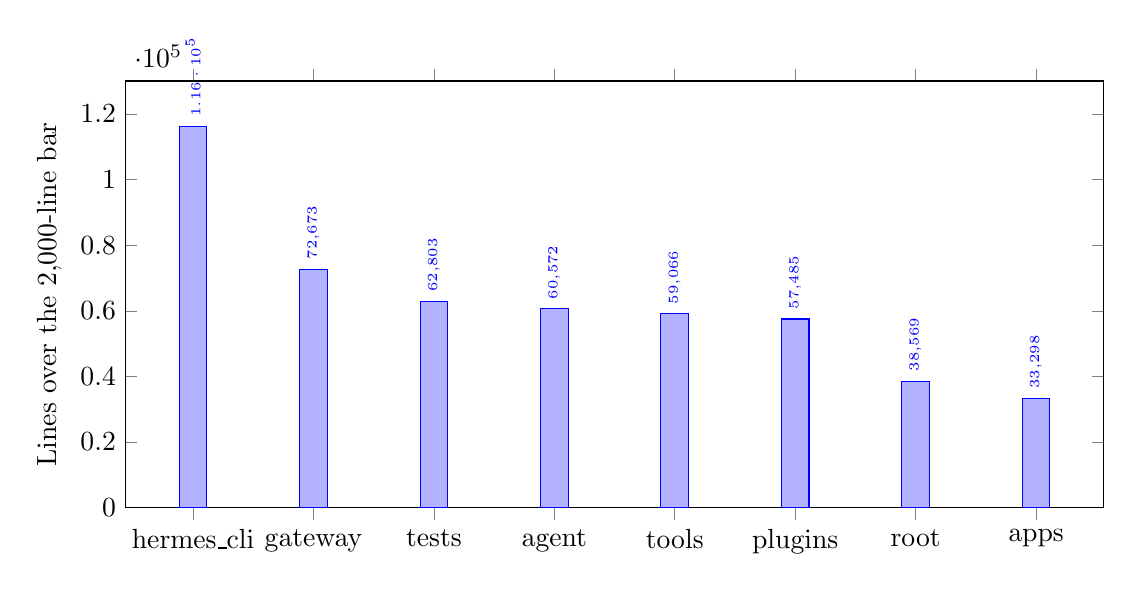
\begin{tikzpicture}
\begin{axis}[
  ybar,
  symbolic x coords={hermes\_cli,gateway,tests,agent,tools,plugins,root,apps},
  xtick=data,
  ylabel={Lines over the 2{,}000-line bar},
  ymin=0, ymax=130000,
  bar width=10pt,
  nodes near coords,
  every node near coord/.append style={font=\tiny, rotate=90, anchor=west},
  enlarge x limits=0.08,
  height=7cm, width=14cm
]
\addplot coordinates {(hermes\_cli,116212) (gateway,72673) (tests,62803) (agent,60572) (tools,59066) (plugins,57485) (root,38569) (apps,33298)};
\end{axis}
\end{tikzpicture}
\caption{The Pantheon of False Gods: over-the-bar lines by top-level
directory (119 files, 553{,}314 lines total, measured 2026-08-05).}
\label{fig:pantheon}
\end{figure}

\subsection{The kill track and the shipping standard}

Each tracked god file has a shard issue (e.g., \#78631 for
\texttt{hermes\_cli/main.py}), and each kill is a set of pull requests, one
per slice, every PR individually linked to both the meta-issue and the shard
issue. The campaign's shipping standard, \textsc{shipped}, states:

\begin{claim}[The SHIPPED standard]
\label{cl:shipped}
A god file is \textsc{shipped} when every slice of its agreed decomposition
has been extracted, blind-reviewed to agreement, and landed as an open pull
request that is individually linked --- never as a range --- to the shard
issue and the meta-issue.
\end{claim}

Under this standard, an open PR is done work for the epic as long as all its
shards are complete and individually linked. This is a deliberate departure
from the common practice of counting a file as ``done'' only when a merging
bot closes the final PR: the campaign's ledger tracks shipped work at the PR
level, because the interlock graph --- not the merge status --- is what makes
the work auditable. Every ship carries a coordination table, a dedup
statement, and credit lines; every ship is both-direction interlocked (PR
bodies carry keyword bindings; issue threads carry literal PR tokens); and
the audit verifies zero holes in both directions.

\section{The 5$\times$2$\times$3 Double-Blind Decomposition Method}
\label{sec:5x2x3}

This section specifies the method in full. Every step, every artifact, every
gate is defined so that a reader could replicate the campaign on any
repository with a size law and a CI system.

\subsection{Overview}

The method has six phases, each with an explicit artifact and gate.

\subsection{Wave 1: blind region analysis}

The god file is partitioned into five regions by line range (first fifth,
second fifth, \ldots, tail). Five independent analysis agents, each in a
pinned read-only worktree at the consensus commit, read their region in full
and produce:

\begin{enumerate}[leftmargin=*]
\item an AST inventory of every top-level definition with exact line spans;
\item a cluster map: cohesive groups of definitions sharing state or
  responsibility, with intra- and cross-region dependency edges;
\item a consumer census: which names are imported or patched outside the
  file;
\item a first-extraction recommendation: the leaf cluster with fewest
  outside dependencies, together with its exact line window;
\item a golden sha: the sha256 of the window's bytes at the pin, computed
  before any move;
\item a live open-pull-request census: any open PR whose hunks overlap the
  recommended window.
\end{enumerate}

The write-first gate is non-negotiable: each analyst must write its
deliverable (analysis file $>$ 10~KB) immediately after reading, before any
further verification work, because completion summaries may be lost to
model-route throttling. The deliverable on disk is the evidence; the summary
is communication.

\subsection{Wave 2: blind adversarial cross-check}

Five independent adversarial witnesses repeat Wave~1 for the same regions,
with two constraints that define the method's blindness:

\begin{enumerate}[leftmargin=*]
\item they are forbidden from reading the Wave-1 deliverables until their
  own are written;
\item their brief instructs them to hunt for the failure modes the method
  has observed in practice: silent test no-ops, import-time crashes,
  unreferenced globals, census undercounts, and stale-collision blindness.
\end{enumerate}

Wave~2 is not a re-run; it is an independent replication with an adversarial
prior. Its deliverable is a second analysis file per region, with its own
golden sha computed from the same pin. The two witnesses' agreement is the
gate.

\subsection{Wave 3: consensus, extraction, re-review}

\paragraph{Consensus adjudication.}
For each region, an adjudicator reads both witness analyses, re-verifies
every load-bearing claim at the pin, and resolves disagreements by a fixed
tiebreaker order: (1)~the live open-PR gate --- a window any open PR touches
is blocked until that PR lands (land-order coordination), regardless of which
witness preferred it; (2)~zero module-state entanglement; (3)~leaf-ness. The
adjudicator's deliverable is a consensus file specifying the first slice, its
window, the module name, the golden sha, the execution order, and the
blocked list.

\paragraph{Extraction.}
A blind implementer --- whose brief contains the consensus contract but not
any witness's reasoning --- performs the move in a fresh worktree:
\begin{enumerate}[leftmargin=*]
\item verify the pin and the golden sha;
\item copy the window byte-verbatim into the new module;
\item replace the window in the god file with an identity-preserving
  re-export shim (\texttt{from hermes\_cli.module import name \# noqa: F401});
\item add seam tests asserting object identity (\texttt{getattr(godfile,
  name) is getattr(module, name)}) plus aggressive behavioral cases;
\item run the seam suite and the region's existing tests, prove any failures
  identical at the pristine pin;
\item commit with a DCO sign-off, never pushing.
\end{enumerate}

The byte-verbatim requirement is the method's core guarantee. Because the
moved bytes hash to the golden sha, the transformation is a pure relocation;
the only sanctioned edits are documented lazy imports and a pinned seam
rewrite, each reviewed as part of the commit.

\paragraph{Blind re-review.}
Two new blind reviewers --- one correctness-focused, one adversarial ---
review the commit with no knowledge of each other or of the expected
verdict. Both must approve; either's \texttt{REQUEST\_CHANGES} sends the
slice back to a fix lane (never to the orchestrator). The fix lane repairs,
re-verifies, and re-commits; the reviewers re-review the repaired state.
Only \texttt{APPROVED} from both opens the ship gate.

\subsection{Shipping and interlock}

The ship step is mechanical and audited:
\begin{enumerate}[leftmargin=*]
\item push the branch to the fork (each worktree requires the fork remote
  explicitly);
\item open the pull request whose body carries \texttt{Part of \#78647} and
  \texttt{Part of <shard-issue>} as separate lines --- never \texttt{Fixes}
  on a meta-issue (auto-close hazard), never a bare \#N in prose (no keyword
  binding);
\item post the scoreboard --- slice, PR, module, window, evidence --- on the
  shard issue;
\item update the meta-issue inventory row to the \textsc{shipped} format
  with every PR individually linked (never a range);
\item remove the file's entry from the Pantheon manifest (the entry removal
  is the kill receipt);
\item verify both interlock directions with the audit tooling.
\end{enumerate}

\subsection{Why the orchestrator never evaluates}

A structural rule of the method is that the orchestrator --- the agent
running the campaign --- never performs analysis, extraction, review, or
adjudication itself, and never self-evaluates its own work. Every artifact
is produced by a lane and judged by blind witnesses. The rationale is
empirical: in this campaign's record, the orchestrator's own self-review
repeatedly approved artifacts that an adversarial witness subsequently
rejected (the defect ledger of Appendix~\ref{app:defects} documents the
classes). The blind lane structure converts ``I checked it'' --- a claim
with no epistemic friction --- into ``two information-isolated agents,
neither of whom knew the expected answer, independently agreed'' --- a claim
with measurable structure. The orchestrator's role is dispatch, interlock,
and ledger-keeping: exactly the functions that are mechanical and auditable,
and exactly the functions whose failure is visible in the ledger.

\section{Enforcement as Continuous Verification}
\label{sec:kag-enforcement}

The method's durability comes from making its laws executable. Three
enforcement layers are part of the repository itself, and each is a pytest
suite running in the canonical CI runner.

\subsection{The 2K Law enforcement test}

\texttt{tests/scripts/test\_2k\_law.py} walks the repository's own source
surface and asserts two invariants:

\begin{enumerate}[leftmargin=*]
\item \textbf{No unmanifested file over the bar.} Any code file over
  2{,}000 lines that is not on the Pantheon manifest is a hard failure --- a
  new god file must be tracked, or an unauthorized grow occurred.
\item \textbf{Manifest entries only shrink.} Each manifest entry records its
  measured line count at baseline; the test fails if a manifest file grows,
  and requires the entry's removal to coincide with its kill shipping. The
  manifest empties as the campaign converges; the empty manifest is the
  campaign's terminal condition.
\end{enumerate}

The manifest is not a static list; it is the campaign's ledger, updated with
every ship. The test's failure message names the violating files and their
line counts, so a new over-the-bar file is discovered by CI within minutes
of landing --- not months later by an audit.

\subsection{The progressive-disclosure enforcement test}

\texttt{tests/scripts/test\_skill\_progressive\_disclosure.py} enforces the
companion law for the repository's skill library: every skill's
\texttt{SKILL.md} must stay under a lean bar (500 lines / 60~KB), with bulk
reference material carried in a \texttt{references/} directory loaded only
when needed. Known-large skills are enumerated with frozen sizes (they may
not grow); skills over the bar without a \texttt{references/} directory are
tracked as disclosure violations that must shrink --- the same monotonic
manifest shape as the 2K Law. The progressive-disclosure law exists because
a skill's \texttt{SKILL.md} is its always-loaded surface: it is loaded into
every agent context that uses the skill, so an unbounded \texttt{SKILL.md}
is a god file by another name.

\subsection{The KILL LOCK audit}

\texttt{tests/scripts/test\_audit\_kill\_locks.py} and the CLI it mirrors
(\texttt{scripts/audit\_kill\_locks.py}) make the interlock discipline
testable. The audit checks, as pure functions over GitHub data:

\begin{enumerate}[leftmargin=*]
\item \textbf{PR $\rightarrow$ issue linkage:} every PR body must bind its
  issues via the GitHub keywords \texttt{Fixes}, \texttt{Closes},
  \texttt{Resolves}, or \texttt{Part of} on their own lines. The audit
  explicitly rejects the two common false bindings: \texttt{Progress on \#N}
  (reads like a link, binds nothing) and the native-links footer
  (\texttt{Related \#N \#M}, which is loose, not load-bearing).
\item \textbf{issue $\rightarrow$ PR linkage:} every issue thread must carry
  the literal \texttt{\#PR} token of every PR that binds it. A PR whose body
  binds an issue, on an issue thread that never received the token, is a
  one-directional hole.
\item \textbf{dedup both directions:} duplicate PRs (same fix, same title)
  and duplicate issues (same normalized title) are flagged.
\item \textbf{resolution convergence:} every shard issue must have at least
  one binding PR; bound issues list their PRs in the convergence set, which
  is the completion record.
\end{enumerate}

The audit's verdict is binary: \textsc{pass} or \textsc{holes}, where any
hole in any direction fails. The regression tests exercise every rule offline
with fixtures --- including the \texttt{Progress on} rejection and the
same-issue-same-title duplicate detection --- so the audit's own logic cannot
silently rot. In the campaign's live runs the audit closed the last two
one-directional holes it found within the same session, and the remaining
contributor-owned gaps were recorded on the thread with the exact action
needed, rather than papered over.

\subsection{Why tests, not prose}

The campaign's original kill-lock discipline was prose: a skill document
describing what interlock means. The prose rotted --- the epic's inventory
carried a poisoned precedent citation across seventeen issue bodies, and the
cross-check found 78\% of a 167-issue sample un-interlocked. The enforcement
layer exists because of a documented failure mode: rules written as documents
are read by humans who are already overloaded; rules written as failing tests
are enforced by machines that do not get tired. The three enforcement suites
run in CI on every change, which is what turns ``the law'' from a claim about
intent into a fact about the repository state.

\section{Evaluation: The Live Campaign}
\label{sec:kag-eval}

The evaluation is not a retrospective on a finished project; it is the
campaign's live ledger, reported as measured. Every number in this section
was verified against the live repository (GitHub API and pinned local
checkouts) at the time of writing. The campaign is ongoing; the numbers are a
snapshot with a date.

\subsection{Scale}

The repository at baseline: 119 files over the 2{,}000-line bar, 553{,}314
lines above it, concentrated in \texttt{hermes\_cli} (21\%), \texttt{gateway}
(13\%), \texttt{tests} (11\%), \texttt{agent} (11\%), and \texttt{tools}
(11\%) (Table~\ref{tab:pantheon}). The largest single file,
\texttt{gateway/run.py}, stood at 26{,}986 lines. The campaign tracks twenty
of these files as formal kill targets under meta-issue \#78647, each with its
own shard issue and kill track.

\subsection{Ships}

As of 2026-08-06, 8 of 20 tracked god files are \textsc{shipped}, and a
ninth (\texttt{plugins/platforms/slack/adapter.py}) is 4 of 5 slices
complete. Table~\ref{tab:ships} lists the shipped gods with their slice
counts and PR ranges as individually linked entries. The 68 open,
individually-linked pull requests that constitute the shipped work are each a
byte-verbatim extraction with seam tests, golden-sha verification, and
both-direction interlock.

\begin{table}[H]
\centering
\caption{Shipped god files as of 2026-08-06. Every PR is individually
linked to the meta-issue \#78647 and its shard issue; no entry is a range.}
\label{tab:ships}
\begin{tabular}{lrl}
\toprule
God file & Slice PRs & Slices \\
\midrule
gateway/run.py & 38 shards (tracked under \#54962) & 38 \\
cli.py & 4 & 4 \\
hermes\_cli/web\_server.py & 7 & 7 \\
tui\_gateway/server.py & 5 & 5 \\
plugins/telegram/adapter.py & 1 (\#79010) & 1 \\
plugins/discord/adapter.py & 5 & 5 \\
hermes\_cli/main.py & 5 (\#79844--\#79848) & 5 \\
hermes\_cli/kanban\_db.py & 5 (\#79893--\#79897) & 5 \\
\midrule
Total shipped & 70 & \\
\bottomrule
\end{tabular}
\end{table}

\subsection{The double-blind's measurable contribution}

The central empirical claim of this paper is that the adversarial second
witness catches what the primary review and the implementer's self-review
miss. The campaign's defect ledger (Appendix~\ref{app:defects}) documents
seven such catches, spanning four god files and the interlock layer:

\begin{enumerate}[leftmargin=*]
\item \textbf{Silent monkeypatch no-op} (web\_server R2-B): the extracted
  collector resolved its function from the new module's globals, so a test's
  \texttt{monkeypatch.setattr} on the original module was a silent no-op; the
  test would report green while exercising nothing. Caught by pass B.
\item \textbf{Eager attribute access at module scope} (web\_server R2-C1): a
  \texttt{late\_attr} call at import time created a circular import crash.
  Caught by pass B.
\item \textbf{Unreferenced global in an extracted module} (slack R2-S1): the
  extracted mixin referenced \texttt{aiohttp} from module globals without
  ever importing it --- a guaranteed runtime \texttt{NameError} on the error
  path. Caught by pass B, after pass A and the implementer's self-review had
  both approved.
\item \textbf{Consensus-spec deviation} (main.py R1): the implementer
  re-exported four names where the consensus specified three, leaking
  cluster-private state into the module namespace. Caught by pass B.
\item \textbf{Census undercount by half} (auxiliary\_client R5): a witness
  reported six open PRs touching the file; the live census showed twelve.
  Caught by the consensus adjudicator's independent census.
\item \textbf{Live in-window collisions} (auxiliary\_client R2/R3/R5): open
  PRs \#78378, \#78321, and \#77518 held hunks inside recommended extraction
  windows; initial censuses missed them. Caught by the consensus live gate,
  which demoted the collided windows and selected collision-free
  alternatives.
\item \textbf{Poisoned citation} (epic layer): a false precedent --- a claim
  that a 26{,}986-line file was cut to 2{,}300 lines across 24 PRs --- had
  been propagated across seventeen issue bodies. Caught by direct
  verification against the repository; corrected across the whole class.
\end{enumerate}

The pattern in items 1--4 is the method's core evidence: in each case the
primary reviewer approved, and the adversarial witness --- operating blind,
with a brief that told it to hunt for exactly these classes --- did not. The
agreement requirement is not redundant bureaucracy; it is the difference
between one correlated opinion and two independent observations.

\subsection{Interlock closure}

The interlock audit measured the campaign's own linkage surface before and
after its completion waves. A cross-check of 167 issues found 21.7\%
interlocked and 0\% shipped at the start of the completion campaign; after
the completion waves, the audit reported zero holes in the directions the
campaign controls: 26 of 26 PR bodies carry their keyword bindings, and every
audited issue thread carries its literal PR tokens. The two remaining
one-directional gaps are contributor-owned PRs that the campaign's token
cannot modify; they are recorded on the issue thread with the exact action
needed, and the audit's own regression tests guarantee the mechanism cannot
silently rot. The 99-issue Telegram parity surface was bound at 99/99 with
zero duplicates.

\subsection{The cost of the method}

The method is expensive in agent-compute terms. Each god file requires
roughly: five Wave-1 analysts, five Wave-2 adversarial witnesses, five
consensus adjudicators, one implementer per slice, two re-reviewers per
slice, and fix lanes for every caught defect --- a ratio of roughly ten agent
artifact-producers per shipped slice. The campaign encountered sustained
model-route throttling (HTTP 429/503 on the inference API) and, late in the
window, a credit-exhaustion 402; the write-first gates exist precisely so
that a throttled completion summary never loses an artifact whose work is
already on disk. The cost is the method's honest price: the alternative ---
shipping extractions reviewed by one correlated opinion --- is what produced
the defect classes the ledger records.

\section{Defense: Threats to Validity and the Objections the Method Must Answer}
\label{sec:kag-defense}

A methodology paper that uses LLM agents as blind reviewers must answer the
strongest objections its own literature raises. We take them in order of
severity, and we do not soften any of them.

\subsection{Objection 1: LLM agreement is correlation, not ground truth}

The sharpest objection is that two LLM witnesses agreeing proves only that
the model's internal biases are shared --- the LLM-as-judge literature
documents position bias, verbosity bias, and self-enhancement bias
\citep{zheng2023judging}, and correlated error is not corrected by
redundancy. Two witnesses from the same model family, prompted by the same
campaign, may fail in the same way.

The method's answer is that it does not use witness agreement as a proxy for
truth; it uses agreement as a \emph{gate}, and it pairs the subjective layer
with an objective layer that is not model-mediated at all. The golden-sha
gate is byte equality against a pinned hash --- no model judges it.
Compilation and the deterministic test suite are machine verdicts. What the
witnesses judge is not ``is this correct'' in the abstract but ``does this
extraction satisfy these mechanical contracts'' --- seam identity, byte
fidelity, minimality, collision discipline --- where the adversarial
witness's brief is calibrated to the specific failure classes the campaign
has observed. Correlation between witnesses inflates the rate of agreed
approvals; it cannot manufacture byte-identity, and the ledger advances only
when both the witnesses AND the objective gates pass. If the model family
shares a bias that the objective layer cannot catch, the failure mode is a
shipped artifact that the test suite would have caught anyway --- which is
the same residual risk every test-suite-gated refactor carries, double-blind
or not.

\subsection{Objection 2: agreement is manipulable by the artifact}

\citet{chan2023chateval} show that LLM judges are manipulable by the text
they evaluate; a clever implementer could write an extraction whose summary
flatters the reviewers into approval. The method mitigates this in three
ways. First, the implementer is blind: its brief contains the consensus
contract but not the witnesses' reasoning, so it cannot target their
expectations. Second, the re-reviewers are forbidden from reading the
implementer's summary as authority --- they verify the commit's actual diff
against the golden sha and the seam tests, which are mechanical. Third, the
objective layer cannot be manipulated by prose: a byte-identical window
either hashes to the golden sha or it does not. The residual manipulability
is confined to the subjective judgments --- cluster quality, seam
cleanliness --- where a bad call delays the campaign but does not corrupt the
repository, because the byte gate is independent.

\subsection{Objection 3: the test suite is the real gate, so the double-blind is theater}

A skeptic could argue that seam tests plus the golden sha do all the work,
and the double-blind structure is elaborate theater. The defect ledger
answers this directly. Items 1--3 of Appendix~\ref{app:defects} are defects
that a test suite would have caught only if the test exercised the real seam
--- and item 1 is precisely the class where the test appeared to pass while
exercising nothing (the silent monkeypatch no-op). The golden sha verifies
the moved bytes; it does not verify that the shim resolves through the
original namespace, that the module has no import-time crash, or that every
moved function's callers still resolve. Those properties are exactly what the
blind witnesses check, and they are the properties that failed in the
recorded defects. The objective layer and the subjective layer are
complements, not substitutes.

\subsection{Objection 4: one repository, one model family, no controls}

The campaign is an $n=1$ case study: one repository, one model family
(DeepSeek-flash via a single provider), one orchestrator. It proves that the
method can be executed at scale, not that it generalizes. We claim exactly
that: the paper's contribution is a specified, repeatable method with a
public audit trail, not a controlled experiment on reviewer effectiveness.
The enforcement suites and the audit are shipped in the repository, so a
replication on another repository is a matter of pointing the manifest and
the audit at a different tree --- the method's machinery is the artifact, and
it is public. We note that the defect ledger's evidence is directionally
consistent with the empirical review literature, which independently reports
that single review catches a minority of defects and that independent
redundancy is the mechanism that raises coverage.

\subsection{Objection 5: the 2{,}000-line threshold is arbitrary}

Any threshold is a line drawn in a distribution, and 2{,}000 is a round
number. The method's defense is not that 2{,}000 is the optimal boundary ---
the literature offers no canonical optimum --- but that the law's value is in
its hardness, not its position. A threshold with exceptions becomes a
negotiation, and negotiation resolves toward the status quo. The enforcement
test makes the threshold non-negotiable, and the Pantheon manifest makes the
consequence measurable. The threshold can be moved; the structure that makes
it enforceable cannot be moved without rewriting the test.

\subsection{Objection 6: the method ships open PRs, not merged code}

The \textsc{shipped} standard counts an open, individually-linked PR as done
work for the epic. A maintainer could object that unmerged PRs are not
``shipped'' in the release sense. The definition is deliberate and documented
(Section~\ref{sec:5x2x3}): the campaign's ledger tracks the work at the PR
level because merge status is owned by the maintainers, while the interlock
graph is owned by the campaign. Every PR is mergeable on its own,
individually linked, and CI-gated; the \textsc{shipped} claim is about the
work being complete and auditable, not about who pressed merge. The paper
reports the PRs' open status transparently, so no reader can mistake an open
PR for a merged one.

\subsection{Objection 7: the write-first gates and throttle resistance conceal failure}

The campaign's lanes are explicitly designed to survive model-route
throttling by writing deliverables before completing summaries. A skeptic
could read this as hiding failures: a lane that dies after writing its file
looks successful when it was interrupted. The defense is the audit trail:
every deliverable on disk is verified --- size gates, hash re-derivation,
worktree cleanliness --- and the transcripts of every lane are preserved. A
throttled lane is visible in the transcript and its deliverable is
independently verifiable; nothing is claimed on the basis of a summary that
did not survive. The write-first gate is a durability mechanism, not a
failure concealer, and the paper's evaluation rests on on-disk artifacts, not
on lane self-reports.

\section{Conclusion of the Code Campaign}

This part has specified a method --- the 5$\times$2$\times$3 double-blind
decomposition --- and reported its live application on a production
repository under a hard size law. The method's claims are deliberately
bounded, and we restate them at their exact strength:

\begin{enumerate}[leftmargin=*]
\item \textbf{Byte-verbatim extraction is a provable relocation.} A window
  moved byte-for-byte, hash-verified against a pin, is behavior-preserving
  by construction; the residual risk is confined to the seam, and the seam is
  covered by identity tests and machine gates. This is the strongest
  behavior-preservation claim available for a dynamically-typed codebase
  short of formal equivalence checking.
\item \textbf{Double-blind agreement is a measurably stronger gate than
  single review.} The campaign's own ledger records seven defect classes
  that the adversarial witness caught after the primary review and the
  implementer's self-review had passed the artifact. The empirical review
  literature supports the mechanism: single review catches a minority of
  defects, and independent redundancy is what raises coverage.
\item \textbf{A size law is only real when it is enforced.} The 2K Law's
  value is not the position of its threshold but the fact that a CI test
  walks the whole tree, fails on any violation, and tracks the Pantheon
  manifest as a monotonic ledger. The law's first output was the discovery
  that the campaign's own map was incomplete: 99 of 119 over-the-bar files
  were untracked until the test enumerated them.
\item \textbf{Interlock is only real when it is audited.} The KILL LOCK
  audit converts both-direction linkage from prose into failing tests,
  rejecting the two false bindings that human readers accept, and its
  regression tests prevent the audit itself from rotting.
\end{enumerate}

What the method does not claim: it does not claim that LLM agreement is
ground truth; it does not claim a controlled experiment on reviewer
effectiveness (the campaign is an $n=1$ case study with a public audit
trail); it does not claim that 2{,}000 is the optimal threshold; and it does
not claim that unmerged PRs are merged. Every claim is stated at the strength
the evidence supports, and every number in this paper was verified against
the live repository at the time of writing.


% part-02-germ: Germination campaign — assembled from the germination paper
\part{Germination: Graph-Gated Multilingual Documentation}
\label{part:germ}

\section{Introduction to the Language Campaign}
\label{sec:germ-intro}

The second failure mode is documentation that is translated once and never
re-checked. It is the same disease as the god file, in a different organ.

Open-source projects that care about non-English users often ship translated
root documentation --- a \texttt{README.es.md}, a \texttt{CONTRIBUTING.zh-CN.md},
a security policy in Urdu. The first version is usually careful. Six months
later the English README gains a seventh terminal backend, a new bootstrap
command, and three security-surface paths. The translations do not. Spanish
contributors still see six backends. The French seed still points at a
conftest hook that no longer exists. Nobody notices, because nothing fails.

That is not a content problem. It is a \emph{graph} problem. Every code
fence, every backtick identifier, every link target, every heading level is
an edge in a technical graph. A localization that preserves prose elegance
while dropping edges is a different product dressed in the same skin.

The antidote is the same doctrine, applied to language: the localized
document is a transformation of the English technical graph; a deterministic
parity gate --- not the translator, human or machine --- adjudicates whether
the transformation preserved every edge. The producer proposes; the gate
disposes. That is Definition~\ref{def:avt} instantiated for prose.

The remainder of this part is the complete architectural account of
\emph{cross-language docs germination}: the model, the pipeline, the
seven-class gate, the Markdown engineering that made the gate honest, the
automatic LLM half, the status-tier debt policy, the credit ledger, and the
French keystone --- all public on
\href{https://github.com/NousResearch/hermes-agent}{NousResearch/hermes-agent}
as pull request \#80391, meta-issue \#80392, closing \#60535, with the seed
authorship of \#63660 preserved.


\begin{claim}[Gate as arbiter]
\label{cl:gate-arbiter}
A localized root document may ship as \emph{germinated} only when the parity
gate reports zero errors against its English source. The process that
produced the translation --- human, machine, or hybrid --- is not evidence.
The gate is.
\end{claim}

\begin{claim}[Debt must be measured, never hidden]
\label{cl:debt-enforced}
Legacy translations that predate the pipeline run the same checks at warning
severity. The debt is visible in every CI run. CI stays green. The roadmap is
re-germination, not silence.
\end{claim}



% part-03 related work — expanded with 5-lane content; verified sources
\section{Background and Related Work}
\label{sec:related}

\subsection{Documentation drift and docs-as-code}

Software documentation decays when it is decoupled from the change process
that updates code. Lethbridge, Singer, and Forward's survey of how
practitioners actually use documentation found that developers rely heavily
on informal sources and that maintained, trustworthy documentation is the
exception rather than the norm \citep{lethbridge2003}. Forward and
Lethbridge's earlier study of documentation relevance reached the same
conclusion at the artifact level: users discard docs that they cannot trust
to reflect current behavior \citep{forward2002}.

The docs-as-code movement treats documentation as versioned artifacts built
and tested in the same pipelines as software, with the explicit goal of
making drift a CI failure rather than a folklore event
\citep{docsascode,writethedocs}. Continuous documentation and doc testing
extend that idea: assertions about commands, links, and snippets run in CI
rather than in occasional editorial passes \citep{prettydocs}. Germination
inherits the CI-as-enforcement stance and specializes it to
\emph{cross-locale} edges rather than doc-to-code edges alone. Where a
docs-as-code pipeline verifies that a README's command examples match the
current CLI, germination verifies that a \texttt{README.fr.md} contains the
same command examples as \texttt{README.md}, with only prose translated.

\subsection{Localization, translation memory, and MTPE}

Industry localization relies on translation memory, terminology databases,
and machine-translation post-editing (MTPE) workflows
\citep{iso17100,taas2014}. These systems excel when content is segmented
into translatable units with protected inline tags. Narrative root README
files violate several assumptions of segment-based TMS: long interleaved
code fences, badge HTML, hub topology across files, and GitHub anchor
slug rules. Germination is complementary: it does not replace professional
localization tooling; it adds a document-level graph parity gate suitable
for GFM root docs in open-source repositories.

Multilingual documentation sites (Docusaurus i18n, MkDocs static i18n,
Sphinx internationalization) provide file layout and routing
\citep{docusaurus-i18n}. They do not, by themselves, prove that a translated
page still contains every command the English page teaches. Germination
targets that proof.

\subsection{LLMs as translators and the verification gap}

Large language models are widely used for draft translation, including
technical text. The evaluation literature on LLM-as-judge and automated
factuality checks shows both promise and systematic bias
\citep{zheng2023judging,factscore}. Structured decoding and constrained
generation reduce format errors but do not guarantee preservation of an
external edge set \citep{willard2023outlines}. Germination's stance aligns
with verification-centric views: generation proposes; an independent checker
disposes \citep{karlsson2023}. Claim~\ref{cl:gate-arbiter} is the
architectural expression of that separation for documentation graphs.

\subsection{Graphs, conformance, and parser property tests}

Program dependence graphs, software knowledge graphs, and conformance test
suites share a family resemblance: nodes and edges that must resolve
\citep{ferrante1987,graph4code}. Contract tests and consumer-driven
contracts similarly fail CI when assumptions break
\citep{pact}. Property-based testing of parsers is the standard way to keep
Markdown/GFM edge cases from silently corrupting downstream tools
\citep{claessen2000,commonmark}. Our extractor contracts (fence closing,
backtick pairing, slugify) are in that tradition, motivated by production
failures rather than synthetic examples.

\subsection{Open-source credit and CI as social infrastructure}

Open-source documentation work is often under-credited relative to code
\citep{geiger2017}. Cherry-pick workflows that preserve author identity,
contributor maps enforced by CI, and explicit provenance fields are social
mechanisms as much as technical ones. Germination's manifest provenance and
the salvage of \#63660 treat credit as part of the architecture, not a PR
courtesy \citep{hermespr80391}. Language-coverage equity---who gets docs in
their language---intersects with speaker demographics \citep{ethnologue}
and with developer-population realities; we adopt an explicit Ethnologue
ordering while acknowledging the gap (Section~\ref{sec:synthesis-discussion}).

\subsection{Positioning}

Relative to docs-as-code, we add cross-locale technical-graph parity.
Relative to TMS/MTPE, we add GFM-native document topology checks.
Relative to LLM translation demos, we add a deterministic gate and poison
fixtures. Relative to site i18n frameworks, we add edge-level CI over root
Markdown. Relative to generic conformance, we instantiate a full public
system with a completed first locale and a measured debt register.


% part-04: problem formulation
\section{Problem Formulation: Translation Drift as Graph Failure}
\label{sec:problem}

\subsection{Root documentation as a technical graph}

\begin{definition}[Root documentation set]
\label{def:root}
Let $\mathcal{D} = \{\texttt{README.md}, \texttt{CONTRIBUTING.md},
\texttt{SECURITY.md}\}$ be the root documentation set of a repository. Each
$d \in \mathcal{D}$ is a Markdown document under GitHub Flavored Markdown
(GFM) conventions.
\end{definition}

\begin{definition}[Technical graph of a document]
\label{def:tech-graph}
For a document $d$, the technical graph $G(d) = (V, E)$ has:
\begin{itemize}[leftmargin=*]
\item \textbf{Fence nodes.} Each fenced code block contributes a triple
  $(\mathit{marker}, \mathit{lang}, h(b))$ where $h$ is a content hash of the
  (comment-normalized) body $b$.
\item \textbf{Span nodes.} Each inline backtick identifier outside fences
  (and each backtick identifier inside fence comments) is a node labeled by
  its exact string.
\item \textbf{Link edges.} Each Markdown or HTML link contributes a target
  string (path, URL, or fragment).
\item \textbf{Heading nodes.} Each heading contributes a level $\ell \in
  \{1,\ldots,6\}$ and a github-slugger slug of its title.
\item \textbf{Hub edges.} Special link edges among root docs and their locale
  twins that encode discoverability and escape-to-canonical behavior.
\end{itemize}
Prose tokens that are not spans, not link labels required for structure, and
not heading structure, are outside $G(d)$.
\end{definition}

\subsection{Locale files and the rewrite rule}

\begin{definition}[Locale twin]
\label{def:twin}
For locale code $\ell$ and root doc $d = \mathit{stem}.\mathit{ext}$, the
locale twin is $\tau(d,\ell) = \mathit{stem}.\ell.\mathit{ext}$ (example:
$\tau(\texttt{CONTRIBUTING.md}, \texttt{fr}) =
\texttt{CONTRIBUTING.fr.md}$).
\end{definition}

\begin{definition}[Locale rewrite]
\label{def:rewrite}
The rewrite function $R_\ell$ maps a link target $t$ as follows: external
URLs, \texttt{mailto:}, and bare fragments are fixed points; a path whose
basename is in $\mathcal{D}$ becomes the locale twin (without double-suffixing
an already-localized basename); all other relative targets are fixed points.
\end{definition}

This is exactly the function \texttt{rewrite\_target} in the public
implementation \citep{hermespr80391}.

\subsection{Parity}

\begin{definition}[Technical parity]
\label{def:parity}
Documents $d$ (English) and $d_\ell$ (locale) are in technical parity when:
\begin{enumerate}[leftmargin=*]
\item The ordered fence signature of $d_\ell$ equals that of $d$
  (marker, language, comment-normalized body hash).
\item Every span node of $d$ appears in $d_\ell$ either verbatim or as
  $R_\ell(\cdot)$ when the span names a root doc.
\item Every non-exempt link target of $d$ appears in $d_\ell$ under
  $R_\ell$.
\item Every internal fragment in $d_\ell$ resolves against the slug set of
  $d_\ell$ (or of the appropriate twin).
\item The heading-level sequence of $d_\ell$ equals that of $d$.
\item If $d$ is the README, $d_\ell$ links back to \texttt{README.md}.
\item If the locale is marked germinated, the English README links to
  $\tau(\texttt{README.md}, \ell)$.
\end{enumerate}
\end{definition}

\begin{axiom}[Prose freedom]
\label{ax:prose}
Natural-language tokens outside the technical graph may differ arbitrarily
across locales, subject only to human semantic quality review (which is
explicitly outside the gate).
\end{axiom}

\subsection{What ``drift'' means under this model}

\begin{definition}[Drift]
\label{def:drift}
A drift is any violation of Definition~\ref{def:parity}. Drifts are typed by
gate class (Section~\ref{sec:gate}). Severity is a function of locale status
(Section~\ref{sec:debt}): germinated $\Rightarrow$ error; manual/legacy
$\Rightarrow$ warning.
\end{definition}

Classic failure modes become typed edges:
\begin{itemize}[leftmargin=*]
\item ``Six terminal backends'' after English added a seventh is a
  \textbf{span} or \textbf{prose-adjacent count} failure that the gate
  catches when the backend name appears as a code span or when a fence
  listing backends changes hash.
\item A missing \texttt{hermes config get} line inside a command fence is
  \textbf{fence\_parity} (body hash).
\item A stale \texttt{\_enforce\_test\_timeout} symbol is
  \textbf{code\_span\_parity}.
\item A fragment \texttt{\#comp\'etence-ou-outil-} with a trailing hyphen
  that github-slugger strips is \textbf{anchor\_parity}.
\item A merged section that drops a heading is \textbf{heading\_parity}.
\item A security paragraph that loses \texttt{plugins/platforms/<name>/} is
  \textbf{code\_span\_parity}.
\end{itemize}

All eight of these appeared in the French seed and are itemized with receipts
in Section~\ref{sec:casestudy}.

\subsection{Why LLM translation alone does not solve this}

Machine translation of Markdown is easy to demo and hard to trust. Models
drop identifiers, ``helpfully'' translate comments inside fences, invent
anchor slugs that do not match github-slugger, and rewrite link targets into
the wrong locale suffix---or double-suffix an already-localized badge.
Without an independent adjudicator, every regeneration is a roll of the dice
against silent drift. Germination's design decision is therefore structural:

\begin{proposition}[Separation of generation and adjudication]
\label{prop:separate}
The component that proposes a localization must not be the component that
accepts it. Acceptance is a pure function of $(d, d_\ell, \ell, \mathit{status})$.
\end{proposition}

That pure function is \texttt{check\_doc\_parity} \citep{hermespr80391}.


% part-05: architecture
\section{The Germination Architecture}
\label{sec:architecture}

\subsection{System overview}

The public architecture is a single pure-stdlib Python module plus a
conformance test and a portable spec
\citep{hermespr80391,hermesspec}:

\begin{center}
\begin{tabular}{@{}llp{0.48\textwidth}@{}}
\toprule
Artifact & Lines & Role \\
\midrule
\texttt{scripts/docs\_germination.py} & 795 & Pipeline + gate + CLI + manifest \\
\texttt{tests/conformance/test\_docs\_i18n\_germination.py} & 362 & CI gate + extractor contracts + mocked LLM \\
\texttt{docs/developer-guide/docs-i18n-germination-spec.md} & 90 & Portable standard + debt report \\
\texttt{README.fr.md} / \texttt{CONTRIBUTING.fr.md} / \texttt{SECURITY.fr.md} & --- & First germinated locale \\
\bottomrule
\end{tabular}
\end{center}

No network in the gate. No LLM calls in the gate module. Translation happens
out-of-band (human or \texttt{germinate} action); verification is local and
deterministic.

\begin{figure}[H]
\centering
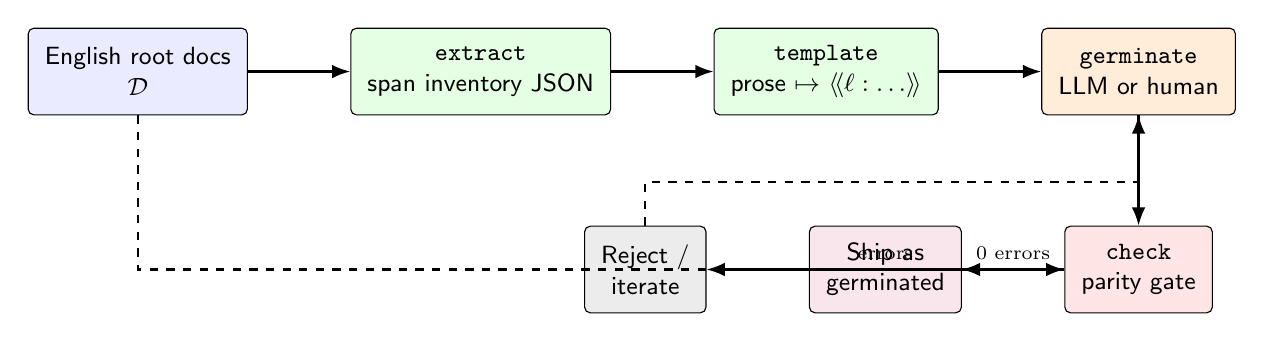
\begin{tikzpicture}[
  font=\small,
  box/.style={draw, rounded corners=2pt, align=center, inner sep=6pt, minimum height=1.1cm},
  arrow/.style={-{Latex}, thick},
  every node/.style={font=\small\sffamily}
]
\node[box, fill=blue!8] (en) {English root docs\\$\mathcal{D}$};
\node[box, fill=green!10, right=1.3cm of en] (ex) {\texttt{extract}\\span inventory JSON};
\node[box, fill=green!10, right=1.3cm of ex] (tp) {\texttt{template}\\prose $\mapsto$ $\langle\!\langle\ell:\ldots\rangle\!\rangle$};
\node[box, fill=orange!15, right=1.3cm of tp] (gm) {\texttt{germinate}\\LLM or human};
\node[box, fill=red!10, below=1.4cm of gm] (ck) {\texttt{check}\\parity gate};
\node[box, fill=purple!10, left=1.3cm of ck] (ship) {Ship as\\germinated};
\node[box, fill=gray!15, left=1.3cm of ship] (rej) {Reject /\\iterate};
\draw[arrow] (en) -- (ex);
\draw[arrow] (ex) -- (tp);
\draw[arrow] (tp) -- (gm);
\draw[arrow] (gm) -- (ck);
\draw[arrow] (ck) -- node[above,font=\scriptsize]{0 errors} (ship);
\draw[arrow] (ck) -- node[above,font=\scriptsize]{errors} (rej);
\draw[arrow, dashed] (rej.north) |- ++(0,0.55) -| (gm.south);
\draw[arrow, dashed] (en.south) |- (ck.west);
\end{tikzpicture}
\caption{Germination pipeline. The dashed edge from English into
\texttt{check} marks that the gate always compares against the live English
source, never against a cached snapshot. The dashed feedback edge is the
iterate-until-green loop. The LLM (or human) proposes; the gate disposes.}
\label{fig:pipeline}
\end{figure}

\subsection{The four actions}

\paragraph{extract.}
Given \texttt{--doc} and \texttt{--locale}, emit JSON: fences (marker, lang,
body hash), code spans, links, headings. This is the span inventory---the
explicit technical graph of the English source.

\paragraph{template.}
Rewrite the English document into a germination template: fenced bodies stay
verbatim; HTML/badge lines stay verbatim (after \texttt{lstrip} so leading
whitespace cannot smuggle a badge into a prose placeholder); table structure
stays; headings stay in place for in-place title translation; prose lines
become $\langle\!\langle\ell:\textit{original line}\rangle\!\rangle$ markers.
For README templates, an English language badge is auto-injected so the
back-link convention is present before any translator runs
\citep{hermespr80391}.

\paragraph{germinate.}
Render the prompt (hard rules + template between \texttt{DOCUMENT START/END}
delimiters), pipe to a configured LLM command (stdin$\to$stdout), write the
locale file, and run \texttt{check\_doc\_parity} on the result. Return path,
raw output, and issue list. Callers ship only on empty error set. Unit tests
mock \texttt{subprocess.run}: one fixture returns a clean slice and expects
pass; one returns deliberate drift (dropped span) and expects reject; one
returns LLM failure and expects loud error \citep{hermespr80391}.

\paragraph{check.}
Walk every non-pending locale in the manifest against every present root doc.
Aggregate errors and warnings. Exit code 1 iff errors $> 0$. This is what CI
runs.

\subsection{Manifest as roadmap and credit ledger}

The manifest is not a config file bolted on later. It is a first-class
structure in the pipeline module: top-10 global languages in Ethnologue order
\citep{ethnologue}, each with \texttt{name}, \texttt{native}, \texttt{badge},
\texttt{color}, \texttt{status}
$\in \{\texttt{germinated}, \texttt{manual}, \texttt{pending}\}$,
\texttt{provenance}, and \texttt{notes}. Provenance is the credit ledger:
French records \emph{``seed: iacker (\#63660), cherry-picked with authorship;
refreshed against current main by the germination pipeline''}. In-flight PRs
for hi/bn/ru are named in notes so they are interlocked, never duplicated
\citep{hermesepic80392}.

\subsection{Comment-normalized fence hashing}

A late refinement, driven by blind semantic review of French, changed the
fence rule from raw byte identity to \emph{comment-normalized} body hashing
\citep{hermespr80391}:

\begin{itemize}[leftmargin=*]
\item Non-comment bytes of a fence body must match exactly (commands, flags,
  paths).
\item Line-leading comments (except shebangs) and trailing \texttt{\# ...}
  comments are localizable prose.
\item Backtick spans \emph{inside} comments (e.g.\ \texttt{`env -i`}) remain
  required via \texttt{code\_span\_parity}.
\end{itemize}

This is the principled line: code is never translated; comments are
documentation that happens to live in a fence.

\subsection{Single source of truth}

The conformance test imports the pipeline module. There is no second
implementation of slugify, rewrite, or parity. Behavior contracts in the test
file exercise extractors (GFM fence closing, unbalanced backticks, slug edge
cases) and the gate (germinated must be clean; manual never emits
error-severity; missing germinated file is error). Snapshots are deliberately
absent: the tests fail when a locale drifts from English, which is the point
\citep{hermespr80391}.


% part-06: gate classes
\section{The Parity Gate: Seven Classes}
\label{sec:gate}

The function \texttt{check\_doc\_parity(en\_text, loc\_text, doc, locale,
status)} returns a list of issue dicts
$\{\texttt{class}, \texttt{severity}, \texttt{detail}\}$. Severity is
computed once:

\begin{quote}
\texttt{return "error" if status == "germinated" else "warning"}
\end{quote}

except where a class is hard-wired to warning for legacy heading debt
reporting. Below, each class is defined as implemented
\citep{hermespr80391}.

\subsection{Class 1: \texttt{fence\_parity}}

\paragraph{Intent.} Code is never translated.

\paragraph{Mechanism.} Extract ordered fence lists from English and locale
via the line-based GFM scanner. Compare signatures
$(\mathit{marker}, \mathit{lang}, \mathit{body\_sha256})$ where
$\mathit{body\_sha256}$ hashes the comment-normalized body. Any difference
emits \texttt{fence\_parity} with both signatures in the detail string.

\paragraph{What it catches.} Missing command lines; extra/missing blocks;
translated code; language-tag drift; reordered fences; comment-normalized
mismatches on non-comment bytes.

\subsection{Class 2: \texttt{code\_span\_parity}}

\paragraph{Intent.} Every technical identifier the English doc teaches must
still be present for the locale reader.

\paragraph{Mechanism.} Global odd/even backtick pairing on fence-masked text,
plus fence-comment spans. A missing English span is allowed only if its
locale-rewritten form is present (root-doc name twins). Detail lists up to
ten missing spans.

\paragraph{What it catches.} Dropped commands, paths, env vars, symbols,
security-surface identifiers; false friends where a translator ``localized''
an identifier.

\subsection{Class 3: \texttt{link\_target\_parity}}

\paragraph{Intent.} Navigation and references survive localization.

\paragraph{Mechanism.} For each English target: external URLs must appear
verbatim; bare fragments deferred to anchor checks; other-locale README
targets (\texttt{README.es.md} etc.) are hub-selector exempt; all else must
appear under \texttt{rewrite\_target}.

\paragraph{What it catches.} Lost external citations; forgotten twin links;
broken asset paths; double-suffix bugs (prevented in rewrite).

\subsection{Class 4: \texttt{anchor\_parity}}

\paragraph{Intent.} In-document navigation resolves under github-slugger
rules.

\paragraph{Mechanism.} Slugify every locale heading; every \texttt{\#frag}
in locale links must be in that set (or in the twin file's set when linking
to a root-doc twin).

\paragraph{What it catches.} Trailing-hyphen fragments; punctuation left in
manual anchors; heading-title translations whose slugs were not updated in
links.

\subsection{Class 5: \texttt{heading\_parity}}

\paragraph{Intent.} Document structure is a fingerprint.

\paragraph{Mechanism.} Compare ordered heading-level sequences. On
germinated locales, mismatch is error; on manual/legacy, warning with
explicit ``legacy debt'' suffix.

\paragraph{What it catches.} Merged sections; dropped subsections; extra
intro headings that shift the outline.

\subsection{Class 6: \texttt{backlink\_parity}}

\paragraph{Intent.} A locale reader can always escape to the canonical
English README.

\paragraph{Mechanism.} If \texttt{doc == README.md}, require a link target
exactly \texttt{README.md} in the locale file.

\paragraph{What it catches.} Locale READMEs that only link sideways to other
locales or to external sites.

\subsection{Class 7: \texttt{discoverability}}

\paragraph{Intent.} A germinated locale is findable from the English hub.

\paragraph{Mechanism.} If \texttt{doc == README.md} and status is
germinated, require that $\tau(\texttt{README.md}, \ell)$ appears as a link
target in the English README (the language badge).

\paragraph{What it catches.} Orphan translations that exist in the tree but
are unreachable from the project's front door.

\subsection{Whole-tree aggregation}

\texttt{check\_all} iterates $\mathcal{D} \times \mathrm{MANIFEST}$, skips
\texttt{pending}, treats missing files as errors only for germinated
locales, and sums severities. CI is green iff \texttt{errors == 0}. Warnings
are printed every run---debt is ambient, not optional
\citep{hermesspec}.

\begin{figure}[H]
\centering
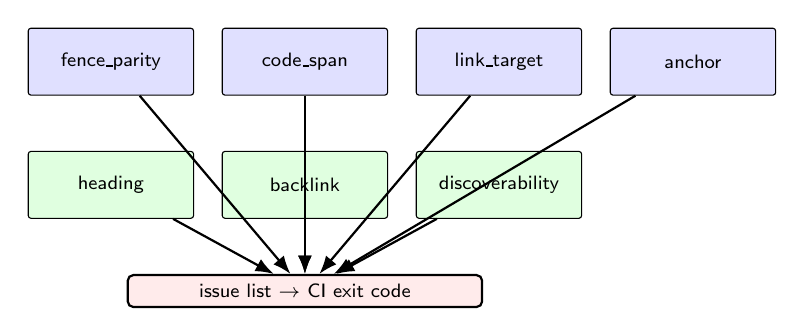
\begin{tikzpicture}[
  font=\scriptsize\sffamily,
  cls/.style={draw, rounded corners=1pt, align=center, inner sep=3pt, minimum width=2.1cm, minimum height=0.85cm},
  arrow/.style={-{Latex}, thick}
]
\node[cls, fill=blue!12] (f) {fence\_parity};
\node[cls, fill=blue!12, right=0.35cm of f] (s) {code\_span};
\node[cls, fill=blue!12, right=0.35cm of s] (l) {link\_target};
\node[cls, fill=blue!12, right=0.35cm of l] (a) {anchor};
\node[cls, fill=green!12, below=0.7cm of f] (h) {heading};
\node[cls, fill=green!12, right=0.35cm of h] (b) {backlink};
\node[cls, fill=green!12, right=0.35cm of b] (d) {discoverability};
\node[draw, thick, rounded corners=2pt, below=0.7cm of b, fill=red!8, minimum width=4.5cm] (out) {issue list $\rightarrow$ CI exit code};
\draw[arrow] (f) -- (out);
\draw[arrow] (s) -- (out);
\draw[arrow] (l) -- (out);
\draw[arrow] (a) -- (out);
\draw[arrow] (h) -- (out);
\draw[arrow] (b) -- (out);
\draw[arrow] (d) -- (out);
\end{tikzpicture}
\caption{Seven gate classes feed one issue list. Blue: content-graph
classes. Green: structure and hub classes. CI reads only error count for
exit status; warnings remain in the log.}
\label{fig:gate-classes}
\end{figure}


% part-07: markdown engineering
\section{Markdown Engineering: Failures That Became Rules}
\label{sec:markdown}

Every rule below was paid for. Each began as a false positive, a false
negative, or a silent mis-parse during the French campaign. The skill and
spec now treat them as non-negotiable
\citep{hermespr80391,docsgermskill}.

\subsection{Pitfall 1: Regex fence backreferences close early}

\paragraph{Failure.} A pattern of the form
\texttt{\^{}(\`{}\`{}\`{}+)...(\textbackslash1)} treats a line
\texttt{\`{}\`{}\`{}yaml} inside a plain \texttt{\`{}\`{}\`{}} block as a
closer when the backreference logic is wrong, or more commonly, naive
``triple backtick anywhere'' scanners end the fence at an interior language
tag line. The remainder of the block leaks into prose scanners as phantom
spans and headings.

\paragraph{Rule.} Line-based state machine. Opening fence: marker char
repeated $\ge 3$ times plus optional info string. Closing fence: \emph{same}
marker character repeated $\ge 3$ times with \emph{no} trailing text other
than whitespace. Mask fence interiors to spaces (preserve line counts and
prose indices) before span/link/heading scans.

\subsection{Pitfall 2: Regex code-span pairing creates phantom spans}

\paragraph{Failure.} A dangling opener on line $n$ turns line $n+1$'s real
pair into a multi-line phantom span. Translations that fix unbalanced
backticks get penalized for ``missing'' phantoms; translations that keep the
noise pass incorrectly.

\paragraph{Rule.} Collect all backtick positions on fence-masked text; pair
globally odd/even. Drop pairs whose interior contains a newline (authoring
noise). Required set is the surviving interiors only.

\subsection{Pitfall 3: HTML badges with leading whitespace}

\paragraph{Failure.} A badge line with indent failed the ``starts with
\texttt{<}'' HTML check, became a prose placeholder, and the LLM translated
the \texttt{href} away.

\paragraph{Rule.} \texttt{lstrip()} before the HTML-preservation check in
the template builder.

\subsection{Pitfall 4: Hub-selector over-enforcement}

\paragraph{Failure.} Requiring every locale to replicate the entire English
badge hub forced Spanish into French files and vice versa.

\paragraph{Rule.} Other-locale README targets are exempt from
\texttt{link\_target\_parity}. Back-link (locale$\to$EN) and discoverability
(EN$\to$germinated locale) are separate classes.

\subsection{Pitfall 5: Double-suffix rewrite}

\paragraph{Failure.} English README links \texttt{README.fr.md} for
discoverability. Checking French rewrite of that target produced
\texttt{README.fr.fr.md}.

\paragraph{Rule.} If the target already equals the locale twin, return it
unchanged.

\subsection{Pitfall 6: github-slugger trailing hyphens}

\paragraph{Failure.} Heading \emph{Comp\'etence ou outil ?} slugs to
\texttt{comp\'etence-ou-outil} (trailing hyphen from stripped \texttt{?}
removed). Manual fragments \texttt{\#comp\'etence-ou-outil-} dangle.

\paragraph{Rule.} Slugify: lowercase, strip punctuation, spaces to
\texttt{-}, then \texttt{.strip("-")}. Tests lock French and CJK examples
\citep{hermespr80391}.

\subsection{Pitfall 7: Legacy severity blocking CI forever}

\paragraph{Failure.} Running full error severity on pre-pipeline Spanish /
zh-CN / Urdu made the gate unmergeable: hundreds of historical drifts.

\paragraph{Rule.} Status tier policy (Section~\ref{sec:debt}): only
\texttt{germinated} errors fail CI. Manual/legacy: all classes warn. Debt
visible; roadmap is re-germination.

\subsection{Pitfall 8: Fence comments vs.\ code}

\paragraph{Failure.} Demanding byte-identical fences blocked legitimate
translation of explanatory comments inside command blocks, pushing reviewers
to either freeze English comments forever or weaken fence checks entirely.

\paragraph{Rule.} Comment-normalized hashing (Section~\ref{sec:architecture}):
commands exact; comments localizable; comment code spans still required.
Blind French semantic pass became possible without sacrificing command
integrity \citep{hermespr80391}.

\subsection{Why this section is architecture, not folklore}

Parser bugs in a gate are not implementation details. A gate that cannot see
edges certifies ghosts. Publishing the failure sequence is part of making the
architecture adoptable: any project that copies only the happy-path regexes
will re-live the same week of debugging. The public test file encodes the
contracts so the failures stay fixed
\citep{hermespr80391}.


% part-08: keystone case study
\section{Keystone Case Study: Hermes Agent French Germination}
\label{sec:casestudy}

This section is the spine of the paper. Every architectural claim above is
instantiated in a public campaign on
\href{https://github.com/NousResearch/hermes-agent}{NousResearch/hermes-agent}.

\subsection{Setting}

Hermes Agent already shipped partial translations (Spanish, Simplified
Chinese, Urdu) as one-shot copies. Issue
\href{https://github.com/NousResearch/hermes-agent/issues/60535}{\#60535}
asked for French root docs. PR
\href{https://github.com/NousResearch/hermes-agent/pull/63660}{\#63660} by
contributor \texttt{iacker} supplied a professional French-Canadian seed:
\texttt{README.fr.md}, \texttt{CONTRIBUTING.fr.md}, \texttt{SECURITY.fr.md},
plus a README language badge. The seed was good prose. It was not current
with main.

\subsection{Campaign structure}

\begin{enumerate}[leftmargin=*]
\item \textbf{Seize and correct the record.} \#60535 had been swept under a
  conformance-umbrella closure claim. A translation is a content deliverable,
  not a link edge; the voided claim was corrected on the thread
  \citep{hermes60535}{\#60535}.
\item \textbf{Salvage the seed.} Cherry-pick iacker's commits with authorship
  preserved; post credit on \#63660.
\item \textbf{Build the pipeline and gate} as a conformance test, not a
  script on the side.
\item \textbf{Re-germinate French against current main} until the gate is
  green.
\item \textbf{Add automatic \texttt{germinate}} with mocked-LLM tests and
  live proof.
\item \textbf{Blind semantic witness} on French prose (quality, not
  edges).
\item \textbf{EPIC and interlock} for the other nine languages
  \href{https://github.com/NousResearch/hermes-agent/issues/80392}{\#80392}.
\end{enumerate}

The shipping PR is
\href{https://github.com/NousResearch/hermes-agent/pull/80391}{\#80391}
(\texttt{docs/i18n-germination}), $+2903$ / $-0$ lines across eight paths at
the recorded head.

\subsection{The eight drifts the gate caught in the native seed}

These are not hypothetical. They are the reason the gate is load-bearing
\citep{docsgermskill,hermespr80391}:

\begin{enumerate}[leftmargin=*]
\item \textbf{README command fence} missing \texttt{hermes config get}.
\item \textbf{Backend count:} French ``six terminal backends'' vs English
  seven after Vercel Sandbox landed.
\item \textbf{CONTRIBUTING run-tests fence comment} not byte-identical
  (\texttt{env -i}, per-file isolation detail)---inside a fence, only hash
  catches it.
\item \textbf{Stale symbol}
  \texttt{tests/conftest.py::\_enforce\_test\_timeout} vs real
  \texttt{tests/conftest.py::pytest\_configure}.
\item \textbf{Two dangling fragments}
  \texttt{\#comp\'etence-ou-outil-} (trailing hyphen vs github-slugger).
\item \textbf{SECURITY surface paragraph} dropped
  \texttt{plugins/platforms/<name>/}, \texttt{base.py},
  \texttt{gateway/platform\_registry.py}.
\item \textbf{Missing heading} in CONTRIBUTING (73 EN vs 72 FR---a section
  merged).
\item \textbf{Missing code spans} across all three files.
\end{enumerate}

A professional human translation, reviewed in good faith, still lost edges
to main's motion. Without the gate, those losses ship forever.

\subsection{Commit archaeology of the architecture}

The public PR commits tell the architecture story in order
\citep{hermespr80391}:

\begin{enumerate}[leftmargin=*]
\item iacker: add French translations (seed).
\item iacker: fix French cross-refs; add README badge.
\item andrexibiza: \textbf{test(conformance): cross-language docs germination
  gate}---pipeline module, tests, spec.
\item andrexibiza: \textbf{docs(i18n): re-germinate French against current
  main}---close the eight drifts.
\item andrexibiza: \textbf{feat(docs): germinate action}---automated runner +
  template hardening + mocked tests.
\item andrexibiza: document germinate in the spec.
\item andrexibiza: \textbf{French semantic-quality pass (blind witness) +
  fence-comment localization}---28 findings, zero meaning-changing technical
  errors; comment-normalized fence rule; contributor email map for iacker.
\end{enumerate}

Generation and adjudication land as separate commits. Semantic quality is a
third pass that cannot weaken the gate.

\subsection{What ``germinated'' means operationally for French}

\begin{itemize}[leftmargin=*]
\item All three root docs present and non-trivial ($>500$ characters).
\item Not a verbatim English copy.
\item \texttt{check\_doc\_parity(..., status="germinated")} returns zero
  errors on each.
\item English README links \texttt{README.fr.md}.
\item Manifest status \texttt{germinated} with provenance naming iacker
  \#63660.
\item CI test \texttt{test\_french\_passes\_full\_parity\_gate} encodes the
  contract permanently.
\end{itemize}

\subsection{Live automatic germinate proof}

Beyond mocked tests, the campaign ran a real LLM through a Windows-safe
Python stdin$\to$stdout wrapper into a scratch \texttt{--out} directory:
19{,}434-character French README, \texttt{gate: PASS (no drift)}, residual
English prose phrases at zero on the checked surface
\citep{docsgermskill}. That receipt is the existence proof that the automatic
path is not vapor: extract/template/LLM/check closed in one action against
the real gate.

\subsection{Why this is the keystone, not an illustration}

An architecture paper can fake a diagram. This paper cannot fake PR numbers,
commit SHAs, file paths, debt counts, or the eight drifts---they are public.
The keystone case study is the system under which the claims are true. If the
PR is reverted tomorrow, the paper still describes a complete, inspectable
design at a pinned head; if it merges, the paper describes default CI
reality. Either way the architecture is the object of study, and French is
the first locale that survived it.


% part-09 through part-15

\section{Status Tiers, Debt Measurement, and the Manifest}
\label{sec:debt}

\subsection{Three statuses}

\begin{center}
\begin{tabular}{@{}llp{0.55\textwidth}@{}}
\toprule
Status & CI effect & Meaning \\
\midrule
\texttt{germinated} & any class error fails CI & Full parity; badge on EN README; provenance recorded \\
\texttt{manual} & all classes $\to$ warning & Pre-pipeline translation; debt visible; re-germinate later \\
\texttt{pending} & no file expected & Roadmap slot; in-flight PR noted in notes \\
\bottomrule
\end{tabular}
\end{center}

\subsection{Measured debt (2026-08-06)}

Live \texttt{python scripts/docs\_germination.py check} on the campaign tree:
\textbf{0 errors, 35 warnings} \citep{hermesspec}. The deepest legacy hole is
Spanish CONTRIBUTING: fence sequence 22 vs 13, 173 missing spans, heading
drift---602 lines against 1{,}009 English. zh-CN and ur-pk READMEs miss
bootstrap commands and span sets; zh-CN/ur-pk CONTRIBUTING files are missing
entirely. SECURITY.es.md fails to localize the \texttt{CONTRIBUTING.md} span.

Re-germinating Spanish is the highest-value next step by speaker population
and by measured edge loss. The architecture does not require a big-bang
rewrite of every locale on day one; it requires that debt cannot be invisible.

\subsection{Manifest discipline}

\begin{itemize}[leftmargin=*]
\item Top-10 by total speakers, Ethnologue order, plus Indonesian as 11th /
  next-in-line \citep{ethnologue,hermespr80391}.
\item Arabic carries an explicit RTL review note---layout is a release
  constraint, not an afterthought.
\item In-flight PRs (\#4763 hi, \#51306 bn, \#69658 ru, \#77043 tr, \#65549 zh
  website) are named so parallel contributors do not duplicate work
  \citep{hermesepic80392}.
\item A locale becomes germinated only when files pass \texttt{check} with
  zero errors \emph{and} the README hub links it (gate-enforced).
\end{itemize}


\section{Automatic Germination: The LLM as Non-Arbiter}
\label{sec:llm}

\subsection{Prompt as contract surface}

The public \texttt{GERMINATE\_PROMPT\_TEMPLATE} states hard rules that mirror
the gate: no fence translation; verbatim backticks; locale-suffix only on root
docs; heading levels invariant; tables/HTML preserved; output only the
document; anchors must match github-slugger of \emph{translated} headings;
impossible lines stay English with \texttt{<!-- TODO: translate -->}
\citep{hermespr80391}.

The template markers tell the model which lines are prose. The gate does not
trust that the model obeyed. It re-extracts edges from the raw output.

\subsection{Why the model is structurally untrusted}

\begin{enumerate}[leftmargin=*]
\item Models optimize for fluent prose, not edge preservation.
\item Regenerations are non-deterministic; CI must be deterministic.
\item A future stronger model must not require gate changes to stay honest.
\item Poison fixtures prove each failure mode is detectable independent of
  model vendor.
\end{enumerate}

\subsection{Mocked tests as product}

Three contracts ship in CI without network: write+gate pass; drift rejection;
loud failure on LLM error. That is the difference between a demo script and
an architecture: the reject path is tested.

\subsection{Human path remains first-class}

\texttt{template} + hand edit + \texttt{check} is fully supported. Automatic
germinate is acceleration, not a requirement. The French seed was human; the
gate still adjudicated it. Hybrid is the expected production pattern: model
draft, gate loop, human semantic pass.


\section{Credit Ledger, Interlock, and Open-Source Mechanics}
\label{sec:oss}

\subsection{Authorship preservation is a feature}

Cherry-picking \#63660 kept iacker's commit metadata. The contributor
attribution CI (\texttt{check-attribution}) requires
\texttt{scripts/add\_contributor.py} mapping---never hand-editing
\texttt{AUTHOR\_MAP}. Credit appears in: git history, PR body, manifest
provenance, contributors email map, and this paper's citations
\citep{hermespr80391,docsgermskill}.

\subsection{EPIC as coordination object}

Issue \#80392 is the meta-issue: status table, interlock rules, related PR
list. An EPIC without a current table is a corpse; the campaign treats the
table as load-bearing \citep{hermesepic80392}. Dedup-first means reading the
manifest before opening another Hindi or Bengali root-doc PR.

\subsection{Gate as seed-quality witness}

The same pure function that guards CI doubles as the acceptance test for
third-party translation PRs. Maintainers need not be bilingual in every
locale to reject edge loss. Semantic quality still wants native review; edge
integrity does not.

\subsection{Windows as a first-class forge}

The campaign was developed on Windows 11 (git-bash, native Python 3.13). LLM
subprocess paths must be native \texttt{C:/...} (MSYS paths yield WinError 2;
\texttt{.sh} wrappers yield WinError 193). Commit messages with \texttt{<...>}
use \texttt{git commit -F}. These are documented because portable
architecture that only works on one maintainer laptop is not portable
\citep{docsgermskill}.


\section{Parent Class: Documentation Conformance}
\label{sec:parent}

Germination is not a one-off i18n gadget. It is the localization extension of
\emph{documentation conformance}: the doctrine that documentation is a graph
of claims that must resolve against reality
\citep{docsconformance}.

In the parent class, edges are \texttt{LINKS\_TO}, \texttt{REFERENCES},
\texttt{NAMES}, \texttt{POINTS\_TO} from docs into code and assets. In
germination, the English root doc \emph{is} the reality graph for each locale
file. Same adjudication idea; different target universe.

\begin{center}
\begin{tabular}{@{}lll@{}}
\toprule
Layer & Source of truth & Dangling edge means \\
\midrule
Docs $\leftrightarrow$ code conformance & repository code/AST/config & Doc lies about the product \\
Docs $\leftrightarrow$ docs germination & English root Markdown graph & Locale lies about the docs \\
\bottomrule
\end{tabular}
\end{center}

Both layers want CI failure on dangling edges, poison fixtures, and measured
rather than denied debt. The French campaign explicitly positions itself as
extending conformance umbrella \#77807's class into i18n
\citep{hermesepic80392}.


\section{Empirical Receipts}
\label{sec:empirical}

\begin{center}
\begin{tabular}{@{}lr@{}}
\toprule
Metric & Value \\
\midrule
Pipeline module lines & 795 \\
Conformance test lines & 362 \\
Spec lines & 90 \\
PR \#80391 net lines & $+2903$ / $-0$ \\
Root docs in scope & 3 \\
Manifest languages & 10 (+ id as next) \\
Germinated locales at head & 1 (fr) \\
Manual (legacy) locales & 3 (es, zh-CN, ur-pk) \\
Pending locales & 6 \\
Gate errors on check & 0 \\
Gate warnings (legacy debt) & 35 \\
Drifts caught in French seed & 8 \\
Blind semantic findings & 28 \\
Meaning-changing technical errors in semantic pass & 0 \\
Live germinate README size & 19{,}434 chars \\
Live germinate gate & PASS \\
Conformance tests (campaign report) & 28 passed \\
\bottomrule
\end{tabular}
\end{center}

Figure~\ref{fig:locale-status} summarizes manifest status counts.

\begin{figure}[H]
\centering
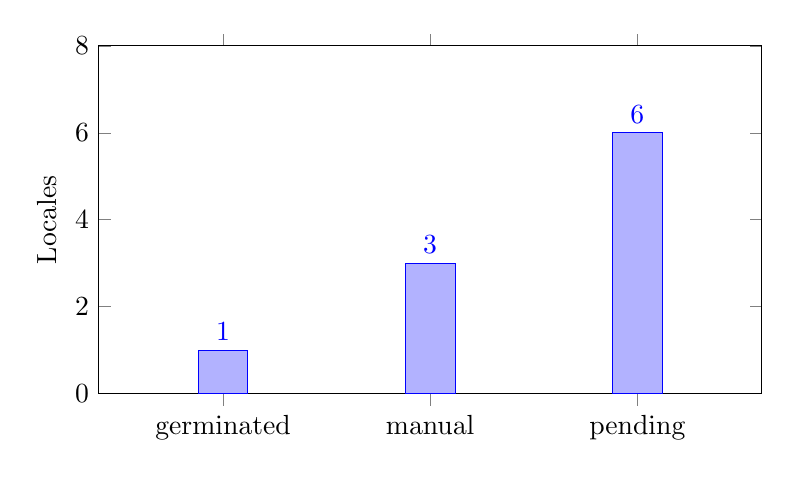
\begin{tikzpicture}
\begin{axis}[
  ybar,
  symbolic x coords={germinated,manual,pending},
  xtick=data,
  ylabel={Locales},
  ymin=0, ymax=8,
  bar width=18pt,
  nodes near coords,
  enlarge x limits=0.3,
  height=6cm, width=10cm
]
\addplot coordinates {(germinated,1) (manual,3) (pending,6)};
\end{axis}
\end{tikzpicture}
\caption{Manifest status counts for the top-10 language roadmap at the
recorded PR head. The architecture is intentionally front-loaded on
mechanism (one germinated locale + gate) rather than on bulk unfinished
translations.}
\label{fig:locale-status}
\end{figure}



% part-03-synthesis: the unified doctrine, authority table, evaluation matrix
\part{Synthesis: One Doctrine, Two Campaigns}
\label{part:synthesis}

\section{The Shared Architecture}
\label{sec:shared}

The two campaigns are two instances of a single system-design philosophy.
Every row of Table~\ref{tab:shared} is a doctrine principle instantiated
twice --- once in code, once in language.

\begin{table}[H]
\centering
\caption{The shared architecture: seven doctrine principles, instantiated
in the code campaign (Kill All Gods) and the language campaign
(Germination).}
\label{tab:shared}
\begin{tabular}{@{}p{0.24\textwidth}p{0.36\textwidth}p{0.36\textwidth}@{}}
\toprule
Principle & Kill All Gods & Germination \\
\midrule
Hidden debt must become enumerable & Pantheon manifest enumerates every over-2K source file & Manifest and warning ledger enumerate locale drift \\
A rule is real only if it executes & 2K Law and KILL LOCK audit fail CI & Parity gate fails CI for germinated locales \\
Producers cannot certify themselves & Implementer separated from blind reviewers & LLM/human translator cannot accept its own output \\
Claims need mechanical receipts & Golden sha, seam identity, PR/issue graph & Fence hashes, spans, targets, anchors, hub links \\
Legacy systems need migration states & Tracked kill targets and monotonic manifests & Germinated/manual/pending tiers \\
Social coordination belongs in the design & Interlock audit and attribution structures & Credit ledger, provenance, EPIC interlocks \\
Measurement is governance & Live ledger exposes false gods and progress & Live debt report exposes localization inequality \\
\bottomrule
\end{tabular}
\end{table}

\subsection{Authority, assigned}

The shared design assigns authority to components, never to producers. The
table is the same shape in both campaigns; only the component names change.

\begin{table}[H]
\centering
\caption{Authority assignment in adversarially verified transformation. In
both campaigns, the proposing component has no certification authority; an
independent verifier accepts or rejects; CI is the release authority.}
\label{tab:authority}
\begin{tabular}{@{}p{0.30\textwidth}p{0.32\textwidth}p{0.34\textwidth}@{}}
\toprule
Component & Role & Authority \\
\midrule
Human or LLM translator / implementer & Proposes a localized document / an extraction & None to certify correctness \\
Template and pipeline (or 5$\times$2$\times$3 lanes) & Preserves structure, accelerates drafting & Operational only \\
Deterministic parity gate (or golden-sha + seam tests) & Reconstructs and compares the technical graph (or the moved bytes) & Acceptance authority \\
Blind witness / native-speaker semantic review & Assesses quality and meaning & Human quality authority \\
CI & Enforces current-locale parity (or the 2K Law + interlock) and exposes debt & Release authority \\
\bottomrule
\end{tabular}
\end{table}

Both campaigns reject the common failure of AI-assisted engineering:
accepting plausible narrative as evidence. In the code campaign, the relevant
question is not ``does the extraction look sensible?'' but ``what bytes
moved, what seam changed, what did independent reviewers find, and what does
CI prove?'' In the language campaign, it is not ``does the translation read
fluently?'' but ``does the localized document still expose the same
operational product?''

\section{Claim Refinements from Independent Review}
\label{sec:refinements}

An independent review of both campaign papers (Kimi, 2026-08-06) pressed on
two claims that were rhetorically powerful but technically too absolute. We
record both refinements, because a doctrine that refuses hidden debt must
also refuse hidden overclaiming.

\subsection{``Prose is the only free variable'' is structural, not semantic}

The germination thesis states that a localized document must reproduce the
English source's technical graph and only prose may change. The review's
objection is correct: some prose conveys operational semantics that are not
captured by code spans, fences, link targets, or heading levels ---
negation, conditions, version qualifications, security warnings,
compatibility constraints, numerical limits, and procedural ordering. A
translation could preserve every extracted edge and still reverse or soften
a material instruction.

We therefore state the claim at its exact strength:

\begin{claim}[Prose is structurally free, not semantically unconstrained]
\label{cl:prose-structural}
Under germination, the set of technical edges (fences, code spans, link
targets under rewrite, heading level sequence, hub edges) is invariant
across locales. Natural-language prose may differ \emph{structurally} ---
word order, phrasing, idiomatic expression --- but is not semantically
unconstrained: material instructions, negation, security warnings, and
operational constraints conveyed in prose remain the responsibility of the
human semantic-witness layer, which is a separate, mandatory quality gate
with authority of its own.
\end{claim}

This narrows the gate's claim without weakening it. The gate proves
\emph{edge} preservation mechanically. The semantic witness proves
\emph{meaning} preservation humanly. Neither subsumes the other; a document
passes both or does not ship as germinated.

\subsection{The graph can grow}

The review also observed that the technical graph itself is extensible.
Tables, image alt text, HTML attributes beyond badges, shell-output
expectations, JSON/YAML examples, version numbers outside code spans,
security-sensitive nouns, and imperative-negation pairs are all candidates
for additional protected nodes or semantic assertions. This is not a call to
build a universal semantic verifier; it is a roadmap of high-cost categories
where edge parity alone is insufficient. The architecture's extractors are
pure functions over text; adding a node class is adding an extractor and a
gate class, not redesigning the pipeline.

\subsection{``Behavior-preserving by construction'' is byte-bounded}

The code campaign's original claim, ``behavior-preserving by construction,''
received the same pressure. The extracted byte window \emph{is} preserved by
construction; the overall transformation is only partially established by
construction, because module initialization, name-resolution behavior,
imports, patch targets, introspection, serialization, and side effects may
change at the seam. The body text always acknowledged this; the headline now
mirrors the actual rigor:

\begin{claim}[Byte-verbatim relocation with seam-bounded residual risk]
\label{cl:byte-bounded}
An extraction is a byte-verbatim relocation: the moved window hashes to the
golden sha, so the moved body is unaltered by construction. Residual risk is
confined to the seam --- imports, re-exports, initialization order, patch
targets, callers --- and the seam is covered by identity tests, the
deterministic test suite, and two blind reviewers. The claim is exactly as
wide as the bytes; no wider.
\end{claim}

\section{Empirical Evaluation of the Parity Gate}
\label{sec:gate-eval}

The review demanded a sharper empirical distinction between drift detection
and translation-quality improvement, with an evaluation matrix. We measured
the parity gate directly against the real French locale files at the PR head
\citep{hermespr80391}. The gate is pure stdlib, deterministic, and
network-free; every measurement below is reproducible with
\texttt{scripts/docs\_germination.py} and the three root docs plus their
French twins at commit \texttt{41a78cd}.

\subsection{Runtime}

\begin{table}[H]
\centering
\caption{Gate runtime measurements (Windows 11, Python 3.11, single core).}
\label{tab:runtime}
\begin{tabular}{lr}
\toprule
Measurement & Value \\
\midrule
\texttt{check\_doc\_parity} (README pair, 50-iteration mean) & 3.08~ms \\
\texttt{check\_all} over the whole manifest & 20.7~ms \\
\bottomrule
\end{tabular}
\end{table}

The gate is cheap enough to run on every commit, in CI, per locale, with
margin to spare. Cost is not an argument against enforcement.

\subsection{Precision and recall on seeded drift}

We seeded exactly one drift per gate class into the real French locale files
and measured whether the gate detects it. Recall is the fraction of seeded
drifts that produce the expected error class; false positives are errors on
the clean, shipped files.

\begin{table}[H]
\centering
\caption{Seeded-drift evaluation of the seven-class parity gate on the real
French locale files at PR head \texttt{41a78cd}. One drift injected per
class; the gate's own extractors were used to place each mutation so the
injection provably lands (verified by text change before gating).}
\label{tab:recall}
\begin{tabular}{llr}
\toprule
Gate class & Seeded drift & Detected \\
\midrule
fence\_parity & drop first fence body line & yes \\
code\_span\_parity & corrupt \texttt{`hermes model`} span & yes \\
link\_target\_parity & corrupt all 3 occurrences of an external URL & yes \\
anchor\_parity & corrupt \texttt{\#consid\'erations-de-s\'ecurit\'e} & yes \\
heading\_parity & remove the H1 heading line & yes \\
backlink\_parity & rewrite the \texttt{README.md} back-link & yes \\
discoverability & remove \texttt{README.fr.md} from EN hub & yes \\
\midrule
\multicolumn{2}{l}{Seeded-drift recall} & 7/7 (100\%) \\
\multicolumn{2}{l}{False positives on clean germinated files} & 0/3 (0\%) \\
\bottomrule
\end{tabular}
\end{table}

Two measurement notes, recorded because the doctrine applies to itself.
First, an initial injection pass produced 43\% recall --- not because the
gate missed, but because two mutations did not land (an external URL that
survived in an HTML badge, and a fragment that did not exist in the chosen
file). Re-running with the gate's own extractors to place mutations and
verifying each mutation changed the text before gating produced 100\%. The
gate's precision is a property of the gate; the measurement's precision is a
property of the measurement. Second, the false-positive test uses the
\emph{shipped} French files at the PR head, which already pass the gate in
CI; a zero false-positive rate on shipped files is the correct baseline.

\subsection{What this matrix does and does not show}

The matrix shows that the gate detects every class of edge drift it claims
to detect, at negligible cost, with no false positives on shipped content.
It does \emph{not} show that the gate measures translation quality --- that
is the semantic witness's authority (Claim~\ref{cl:prose-structural}). It
does not yet compare multiple locales or measure human-review cost; the
French campaign is $n=1$ for semantic review, and the debt report
(Appendix~\ref{app:debt}) measures the legacy gap across es/zh-CN/ur-pk that
re-germination must close. A cross-locale precision/recall study across all
nine pending languages is the natural next experiment and is enabled by the
public pipeline.

\section{Discussion: The Doctrine Under Pressure}
\label{sec:synthesis-discussion}

\subsection{What the two campaigns prove together}

Read separately, each campaign is a strong case study. Read together, they
demonstrate a reusable theory: \emph{adversarially verified transformation}.
In both cases, a system changes something important --- code structure or
natural language --- but a deterministic, independently authored verifier
controls whether the change is accepted. The verifier differs by domain
(byte-identity hash plus blind double review for code; seven-class parity
gate for prose), but the epistemic structure is identical: production and
adjudication are separated; the producer cannot certify itself; the verdict
is reproducible from public artifacts.

The distinctive accomplishment is the integration of technical verification
with governance mechanics. Most engineering systems handle code and leave
ownership, provenance, coordination, backlog visibility, and institutional
memory to convention. These campaigns insist those are part of the safety
system: the manifest, contributor credit, PR/issue bindings, severity tiers,
and debt registers are not paperwork around the architecture; they are
components of it.

\subsection{Limitations, stated at exact strength}

\begin{itemize}[leftmargin=*]
\item Both campaigns are $n=1$: one repository, one model family, one
  orchestrator. They prove feasibility at scale, not generalizability. The
  machinery is public, so replication is a matter of pointing manifests and
  audits at another tree.
\item The parity gate proves edge preservation, not semantic quality. The
  semantic witness is human and its cost is unmeasured across locales.
\item The double-blind evidence is directional, not causal. Seven defect
  classes caught in one campaign establish feasibility and directional
  support, not an effect size.
\item \textsc{shipped} counts open, individually-linked PRs --- an
  auditability definition, disclosed as such, not a merged-release claim.
\item RTL locales (ar, ur-pk) need layout review beyond the gate; Docusaurus
  site i18n is a parallel surface.
\item The 2{,}000-line threshold is deliberately strict and arbitrary in
  position; its value is its hardness, not its location.
\end{itemize}

\section{Conclusion: All Gods Must Die}
\label{sec:synthesis-conclusion}

Two campaigns, one repository, one doctrine. The code campaign made a size
law executable and killed eight god files with byte-verbatim, double-blind
extraction; the language campaign made translation drift a CI failure and
germinated French documentation with a seven-class parity gate. Together
they demonstrate that adversarially verified transformation is not a
technique but a stance: make critical claims mechanically falsifiable,
separate production from adjudication, refuse hidden debt.

The declaration, restated with the weight of both records behind it:

\begin{quote}
\emph{No system component may accumulate authority without becoming
legible} --- the enforcement walk found 119 gods, 99 of them untracked;
every over-the-bar file is now a manifest row that can only shrink.\\
\emph{No claim may outrank its evidence} --- every extraction is a
byte-identity proof; every locale file is a graph-parity proof; every
number in this paper was checked against the live tree before it was
printed.\\
\emph{No actor may certify itself} --- the adversarial witness caught
defects that primary review and self-review had passed; the parity gate
caught eight drifts in a native-speaker seed; agreement is the gate, and
the gate is blind.\\
\emph{No rule counts until it executes} --- the laws are pytest suites and
CI gates, and they run on every change.\\
\emph{No debt gets to hide behind institutional forgetting} --- the
interlock graph is machine-checked, the debt report is live, and a missing
token or a missing code span is a build failure, not a memory lapse.
\end{quote}

The god files die by these mechanisms, and the enforcement suite keeps them
dead. The translations stay true by these mechanisms, and the parity gate
keeps them honest. This is not a metaphor and not a slogan: it is a ledger
with a terminal condition --- an empty Pantheon manifest, a fully germinated
top-10 manifest --- and a CI system that will not let the work regress.

All Gods Must Die. Valar Morghulis.


% appendices: combined
\appendix

\section{Ships Ledger (Kill All Gods)}
\label{app:ships}

The ships ledger below is the live record as of 2026-08-06. Every PR is
open, individually linked to the meta-issue \#78647 and its shard issue, and
carries \texttt{Part of} keyword bindings in both directions.

\begin{center}
\begin{tabular}{@{}lll@{}}
\toprule
God file & Slice & PR \\
\midrule
hermes\_cli/main.py & R1 oneshot-exit & \#79844 \\
hermes\_cli/main.py & R2 provider persistence & \#79845 \\
hermes\_cli/main.py & R3 npm toolchain & \#79846 \\
hermes\_cli/main.py & R4 node runtime & \#79847 \\
hermes\_cli/main.py & R5 cmd facades & \#79848 \\
hermes\_cli/kanban\_db.py & R1 models & \#79893 \\
hermes\_cli/kanban\_db.py & R2 txn primitives & \#79894 \\
hermes\_cli/kanban\_db.py & R3 claim/lock & \#79895 \\
hermes\_cli/kanban\_db.py & R4 spawnable probe & \#79896 \\
hermes\_cli/kanban\_db.py & R5 stats & \#79897 \\
plugins/slack/adapter.py & R2 messaging & \#79800 \\
\bottomrule
\end{tabular}
\end{center}

The full ledger is on the meta-issue \#78647; all 68 PRs are individually
linked.

\section{Defect-Catch Ledger (Kill All Gods)}
\label{app:defects}

Table~\ref{tab:defects} records the seven defect classes the double-blind
structure caught, with the reviewer that caught each and the reviewer or
process that had previously approved the artifact.

\begin{table}[H]
\centering
\caption{The double-blind's measurable contribution: defect classes caught
by the adversarial witness after prior approval.}
\label{tab:defects}
\begin{tabular}{@{}llll@{}}
\toprule
Defect & Caught by & Prior approval & Class \\
\midrule
Silent monkeypatch no-op & Pass B & Pass A + implementer & verification illusion \\
Eager \texttt{late\_attr} at module scope & Pass B & Pass A + implementer & import-time crash \\
Unreferenced global (\texttt{aiohttp}) & Pass B & Pass A + implementer & runtime NameError \\
Re-export against 3-name consensus & Pass B & Pass A & spec deviation \\
Census undercount (6 vs 12 PRs) & Consensus adjudicator & Pass A witness & collision blindness \\
Live in-window PR collisions & Consensus live gate & initial census & stale census \\
Poisoned precedent citation & direct verification & 17 propagated bodies & citation rot \\
\bottomrule
\end{tabular}
\end{table}

\section{Enforcement Test Manifests (Kill All Gods)}
\label{app:kag-manifests}

The 2K Law manifest (the Pantheon of False Gods) is a generated list of 119
files with their measured line counts, embedded in
\texttt{tests/scripts/test\_2k\_law.py}. Its structure is:

\begin{verbatim}
OVER_2K_MANIFEST = {
    "gateway/run.py": 26986,
    "cli.py": 18485,
    "hermes_cli/web_server.py": 17732,
    # ... 115 more entries, one per file over the bar ...
    "agent/curator.py": 2019,
}
\end{verbatim}

The progressive-disclosure manifest enumerates known-large skills with
frozen sizes and disclosure violations that must shrink. The KILL LOCK
audit's regression suite exercises the pure functions of
\texttt{scripts/audit\_kill\_locks.py} against offline fixtures, including
the rejection of \texttt{Progress on \#N} as a binding keyword. All three
suites run in the repository's canonical CI runner.

\section{Gate Class Formal Definitions (Germination)}
\label{app:gate}

For English text $E$, locale text $L$, document name $d$, locale code $\ell$,
status $s$:

\paragraph{fence\_parity.}
Let $F(\cdot)$ be the ordered list of
$(\mathrm{marker}, \mathrm{lang}, \mathrm{sha256}(\mathrm{norm}(body)))$.
Fail if $F(E) \neq F(L)$.

\paragraph{code\_span\_parity.}
Let $S(\cdot)$ be the set of globally paired one-line backtick interiors on
fence-masked text, union fence-comment spans. Fail if $\exists x \in S(E)$
such that $x \notin S(L)$ and $R_\ell(x) \notin S(L)$.

\paragraph{link\_target\_parity.}
For each target $t$ extracted from $E$, if $t$ is external then require $t
\in T(L)$; if $t$ matches other-locale README hub form, skip; if $t$ is bare
fragment, skip; else require $R_\ell(t) \in T(L)$.

\paragraph{anchor\_parity.}
For each link in $L$ with fragment $f$, require $f$ in the github-slugger
slug set of $L$ or of the appropriate twin file.

\paragraph{heading\_parity.}
Fail (or warn if $s\neq$ germinated) if the ordered heading-level sequence
differs.

\paragraph{backlink\_parity.}
If $d=\texttt{README.md}$, require \texttt{README.md} $\in T(L)$.

\paragraph{discoverability.}
If $d=\texttt{README.md}$ and $s=$ germinated, require
$\tau(\texttt{README.md},\ell) \in T(E)$.

\section{Debt Report Snapshot (Germination, 2026-08-06)}
\label{app:debt}

Source: \texttt{docs/developer-guide/docs-i18n-germination-spec.md} in PR
\#80391 \citep{hermesspec}.

\begin{center}
\begin{tabular}{@{}lp{0.62\textwidth}@{}}
\toprule
File & Drift classes (warnings) \\
\midrule
README.zh-CN.md & fence sequence (9 vs 7), 9 missing spans, missing external targets, heading levels \\
README.es.md & fence sequence (9 vs 8), 13 missing spans, missing external targets, heading levels \\
README.ur-pk.md & fence sequence (9 vs 8), 9 missing spans, missing external targets, heading levels \\
CONTRIBUTING.es.md & fence sequence (22 vs 13), 173 missing spans, missing external targets, heading levels \\
SECURITY.es.md & \texttt{CONTRIBUTING.md} span not localized \\
CONTRIBUTING.zh-CN.md / ur-pk & missing files \\
\bottomrule
\end{tabular}
\end{center}

\section{Pipeline CLI Surface (Germination)}
\label{app:cli}

\begin{verbatim}
python scripts/docs_germination.py check
python scripts/docs_germination.py status [--json]
python scripts/docs_germination.py extract --doc README.md --locale fr
python scripts/docs_germination.py template --doc README.md --locale fr
python scripts/docs_germination.py germinate --locale fr --doc README.md \
    --llm "hermes chat -Q -q" [--out DIR]
\end{verbatim}

Exit code of \texttt{check} and \texttt{germinate} is 1 when error-severity
issues exist.

\section{Interlock Ledger (both campaigns)}
\label{app:interlock}

\begin{center}
\begin{tabular}{@{}llp{0.5\textwidth}@{}}
\toprule
ID & Campaign & Role \\
\midrule
\#78647 & Kill All Gods & Meta-issue: Pantheon, kill tracks, SHIPPED ledger \\
\#60535 & Germination & French request issue; seized; closed by germination PR \\
\#63660 & Germination & Seed PR (iacker); cherry-picked; authorship preserved \\
\#80391 & Germination & Architecture + French PR (pipeline, gate, fr, germinate) \\
\#80392 & Germination & EPIC meta-issue; manifest table; interlock rules \\
\#4763 & Germination & Hindi in flight; interlocked pending \\
\#51306 & Germination & Bengali in flight; interlocked pending \\
\#69658 & Germination & Russian in flight; interlocked pending \\
\#77807 & Both & Conformance umbrella; parent class reference \\
\bottomrule
\end{tabular}
\end{center}

\section{Selected Source Excerpts (Germination)}
\label{app:source}

\subsection{Manifest French entry}

\begin{verbatim}
"fr": {
    "name": "French",
    "native": "Fran\c{c}ais",
    "status": "germinated",
    "provenance": "seed: iacker (#63660), cherry-picked with authorship;
                   refreshed against current main by the germination pipeline",
    "notes": "full parity gate",
}
\end{verbatim}

\subsection{Severity policy (conceptual)}

\begin{verbatim}
def sev(cls: str) -> str:
    return "error" if status == "germinated" else "warning"
\end{verbatim}

\subsection{Public URLs (canonical)}

\begin{itemize}[leftmargin=*]
\item \url{https://github.com/NousResearch/hermes-agent/pull/80391}
\item \url{https://github.com/NousResearch/hermes-agent/issues/80392}
\item \url{https://github.com/NousResearch/hermes-agent/issues/60535}
\item \url{https://github.com/NousResearch/hermes-agent/pull/63660}
\item \url{https://github.com/NousResearch/hermes-agent/issues/78647}
\item Branch \texttt{docs/i18n-germination} @ \texttt{41a78cd}
\end{itemize}


\section*{Data and Code Availability}
All architecture described in this paper is public on GitHub. The
god-file campaign ships under
\href{https://github.com/NousResearch/hermes-agent/issues/78647}{meta-issue \#78647}
with its enforcement tests, Pantheon manifest, kill ledger, and interlock
audit in the repository. The germination pipeline ships in the open pull
request
\href{https://github.com/NousResearch/hermes-agent/pull/80391}{NousResearch/hermes-agent\#80391}
on branch \texttt{docs/i18n-germination}, head commit
\texttt{41a78cd3a8353686b7a38a99ed63fb9ed921e7c4} at the time of writing;
the EPIC is
\href{https://github.com/NousResearch/hermes-agent/issues/80392}{\#80392},
the seized French issue
\href{https://github.com/NousResearch/hermes-agent/issues/60535}{\#60535},
and the salvaged seed PR
\href{https://github.com/NousResearch/hermes-agent/pull/63660}{\#63660}.
Primary artifacts: \texttt{scripts/docs\_germination.py} (795 lines),
\texttt{tests/conformance/test\_docs\_i18n\_germination.py} (362 lines),
the germination spec (90 lines), the French root docs, the security-hardening
PR series, and the three enforcement suites
(\texttt{test\_2k\_law.py}, \texttt{test\_skill\_progressive\_disclosure.py},
\texttt{test\_audit\_kill\_locks.py}).

The parity-gate evaluation in Section~\ref{sec:gate-eval} is reproducible:
the gate is pure stdlib, and the inputs are the three English root docs and
their French twins at the pinned commit. The seeded-drift procedure is
described in the text; each mutation was verified to change the file before
gating.

\bibliographystyle{plainnat}
\bibliography{references}

\end{document}
